\graphicspath{{Chapter2/Figs/}}

\section{Multi-Omics Factor Analysis}

The work described in this chapter results from a collaboration with Wolfgang Huber's group at the EMBL (Heidelberg, Germany). It has been peer-reviewed and published in \cite{Argelaguet2018}.

The method was conceived by Florian Buettner, Oliver Stegle and me. I performed most of the mathematical derivations and implementation, but with significant contributions from Damien Arnol and Britta Velten. The CLL data application was led by Britta Velten whereas the single-cell application was lead by me, but with joint contributions in either cases. Florian Buettner, Wolfgang Huber and Oliver Stegle supervised the project.\\
The article was jointly written by Britta Velten and me, with contributions from all authors.


\subsection{Model description} \label{mofa:model_description}
MOFA is a multi-view generalisation of traditional Factor Analysis to $M$ input matrices (or views) based on the framework of Group Factor Analysis (discussed in \Cref{section_gfa}).\\
The input data consists on $M$ views $\bfY^m \in \R^{N \times D_m}$ with non-overlapping features that often represent different assays. However, there is flexibility in the definition of views.\\
Formally, the input data is factorised as:
\begin{equation} \label{mofa_master_equation}
	\mathbf{Y}^m = \mathbf{Z}\mathbf{W}^{mT} + \bepsilon^m
\end{equation}
where $\bfZ \in \R^{N \times K}$ is a matrix that contains the factor values and $\bfW^m \in \R^{D_m \times K}$ are a set of $M$ matrices (one per view) that contain the weights that relate the high-dimensional space to the low-dimensional latent representation. Finally, $\bepsilon^m \in \R^{D_m}$ captures the residuals, or the noise, which is assumed to be normally distributed and heteroskedastic:
\begin{equation}
	p(\epsilon^{m}_{d}) = \Ndist{\epsilon^{m}_{d}}{0,1/\tau_{d}^{m}}
\end{equation}
Non-gaussian noise models can also be defined (see \Cref{section:mofa_ngaussian}), but unless otherwise stated, we will always assume Gaussian residuals.\\
Altogether, this results in the following likelihood:
\begin{equation}
	p(\bfY|\bfW,\bfZ,\bTau) = \prod_{m=1}^{M} \prod_{d=1}^{D_m} \prod_{n=1}^{N} \Ndist{y_{nd}^m}{\bfz_{n}^T\bfw_{d}^{m},1/\tau_d^m}
	% p(y_{nd}^m) = \Ndist{y_{nd}^m}{\bfz_{n,:}\bfw_{d,:}^{mT},1/\tau_d^m},
\end{equation}

Notice that the mathematical formulation so far is equivalent to the Group Factor Analysis described in \Cref{section_gfa}.

\subsubsection{Prior distributions for the factors}  \label{section:mofa_factors}
For the factors, we define an isotropic Gaussian prior, as commonly done in most factor analysis models:
\begin{equation}
	p(z_{nk}) = \Ndist{z_{nk}}{0,1}
\end{equation}
This effectively  assumes (1) a continuous latent space and (2) independence between samples and factors. 

\subsubsection{Prior distributions for the weights}  \label{section:mofa_weights}
The key determinant of the model is the regularization used on the prior distributions for the weights. Here we encode two levels of sparsity, a (1) view- and factor-wise sparsity and (2) an individual feature-wise sparsity. The aim of the factor- and view-wise sparsity is to disentangle the activity of factors to the different views, such that the weight vector $\bfw_{:,k}^m$ is shrunk to zero if the factor $k$ does not explain any variation in view $m$. \\
In addition, we place a second layer of sparsity which encourages inactive weights on each individual feature. Mathematically, we express this as a combination of an Automatic Relevance Determination (ARD) prior \cite{Mackay1996} for the view- and factor-wise sparsity and a spike-and-slab prior \cite{Mitchell1988} for the feature-wise sparsity:
% \begin{equation*}
% 	p(w_{dk}^{m}) = (1-\theta_{k}^{m}) \mathds{1}_0(w_{dk}^{m}) + \theta_{k}^{m} \Ndist{w_{dk}^{m}}{0, 1 / \alpha_{k}^{m}}
% \end{equation*}
However, this formulation of the spike-and-slab prior contains a Dirac delta function, which makes the inference procedure troublesome. To solve this we introduce a re-parametrization of the weights $w$ as a product of a Gaussian random variable $\hat{w}$ and a Bernoulli random variable $s$, \cite{Titsias2011} resulting in the following prior:
\begin{equation}
	p(\hat{w}_{dk}^m,s_{dk}^m) &= \Ndist{\hat{w}_{dk}^m}{0, 1/\alpha_k^m}  \text{Ber}(s_{dk}^m \,|\,\theta_k^m)
\end{equation}
In this formulation $\alpha_k^m$ controls the activity of factor $k$ in view $m$ and $\theta_k^m$ controls the corresponding fraction of active weights (i.e. the sparsity levels).\\

Finally, we define conjugate priors for $\theta$ and $\alpha$:
\begin{align}
	p(\theta_k^m) &= \Bdist{\theta_k^m}{a_0^\theta,b_0^\theta}\\
	p(\alpha_k^m) &= \Gdist{\alpha_k^m}{a_0^\alpha, b_0^\alpha}
\end{align}
with hyper-parameters $a_0^\theta,b_0^\theta =1$ and $a_0^\alpha, b_0^\alpha=1e^{-5}$ to get uninformative priors. Posterior values of $\theta_k^m$ close to $0$ implies that most of the weights of factor $k$ in view $m$ are shrinked to $0$ (sparse factor). In contrast, a value of $\theta_k^m$ close to $1$ implies that most of the weights are non-zero (non-sparse factor). A small value of $\alpha_k^m$ implies that factor $k$ is active in view $m$. In contrast, a large value of $\alpha_k^m$ implies that factor $k$ is inactive in view $m$.

All together, the joint probability density function of the model is given by
\begin{align}
	\begin{split}
	p(\bfY,\hat{\bfW},\bfS,\bfZ,\btheta, \balpha, \btau)  = &\prod_{m=1}^{M} \prod_{n=1}^{N} \prod_{d=1}^{D_m} \Ndist{y_{nd}^m}{\sum_{k=1}^{K} s_{dk}^m \hat{w}_{dk}^m z_{nk},1/\tau_d} \\
	& \prod_{m=1}^{M}\prod_{d=1}^{D_m} \prod_{k=1}^{K} \Ndist{\hat{w}_{dk}^m}{0,1/\alpha_k^m} \text{Ber}(s_{d,k}^m|\theta_k^m) \\
	& \prod_{n=1}^{N} \prod_{k=1}^{K} \Ndist{z_{nk}}{0,1} \\
	& \prod_{m=1}^{M} \prod_{k=1}^{K} \Bdist{\theta_k^m}{a_0^\theta,b_0^\theta} \\
	& \prod_{m=1}^{M} \prod_{k=1}^{K} \Gdist{\alpha_k^m}{a_0^\alpha, b_0^\alpha} \\
	& \prod_{m=1}^{M} \prod_{d=1}^{D_m} \Gdist{\tau_d^m}{a_0^\tau,b_0^\tau}.
	\label{likelihood}
	\end{split}
\end{align}
and the corresponding graphical model is shown in \Cref{fig:MOFA_graphical_model}. This completes the definition of the MOFA model.

\subsubsection{Interpretation of the factors}
Each factor ordinates cells along a one-dimensional axis centered at zero. Samples with different signs indicate opposite phenotypes, with higher absolute value indicating a stronger effect. Intuitively, their interpretation is similar to that of principal components in PCA.\\
For example, if the $k$-th factor captures the variability associated with cell cycle, we could expect cells in the Mitosis state to be at one end of the factor (irrespective of the sign, only the relative positioning being of importance). In contrast, cells in G1 phase are expected to be at the other end of the factor. Cells with intermediate phenotype, or with no clear phenotype (for example if no cell cycle genes are profiled), are expected to be located around zero.

\subsubsection{Interpretation of the weights}
The weights provide a score for each gene on each factor, and are interpreted in a similar way as the factors. Genes with no association with the factor are expected to have values close to zero, as specified by the prior. In contrast, genes with strong association with the factor are expected to have large absolute values. The sign of the loading indicates the direction of the effect: a positive loading indicates that the feature is more active in the cells with positive factor values, and viceversa. \\
Following the cell cycle example from above, genes that are upregulated in the M phase are expected to have large positive weights, whereas genes that are downregulated in the M phase (or, equivalently, upregulated in the G1 phase) are expected to have large negative weights.

% \subsubsection{Interpretation of the noise}
% The use of a probabilistic framework allows the model to explicitly disentangle the signal (the explained variance) from the noise (the unexplained variance). As a rule of thumb, the larger the value of $\tau_d^m$, the higher the explained variance the feature $d$ in view $m$. In contrast, small values of $\tau_d^m$ are indicative of low predictive power by the model.


\subsubsection{Missing values} \label{section:mofa_missing_values}
The probabilistic formulation naturally accounts for incomplete data matrices, as missing observations do not intervene in the likelihood. In practice, we implement this using memory-efficient binary masks $\mathcal{O}^m \in \mathbb{R}^{N\times D_m}$ for each view $m$, such that $\mathcal{O}_{n,d} = 1$ when feature $d$ is observed for sample $n$, 0 otherwise. 

\subsection{Downstream analysis} \label{mofa:downstream}

Once trained, the MOFA model can be queried for a set of downstream analysis (\Cref{fig:MOFA}):
\begin{itemize}
	\item \textbf{Variance decomposition}: calculate the variance explained ($R^2$) by each factor in each view. This is the first and arguably the most important plot to be inspected once the model is trained, as it summarises the variation (i.e. the signal) in a complex multi-view data set using a simple heatmap. With a quick visual inspection, this plot can be used to determine which factors are shared between multiple data modalities and which ones are exclusive to a single data modality.

	\item \textbf{Ordination of the samples in the latent space}: as in any latent variable model, the samples can be visualised in the latent space using scatterplots or beeswarm plots. As we will demonstrate, simply by colouring or shaping the samples in the factor space using external covariates one can easily characterise the etiology of some of the factors.

	\item \textbf{Inspection of weights}: the feature weights can be interpreted as an importance score for each feature on each factor. Inspecting the top weights for a given factor can help to reveals the molecular signatures that underlie each factor.

	\item \textbf{Association analysis between factors and external covariates}: multi-omic data sets typically consist on a large set of molecular readouts that are used for model training, and a small set of additionals covariates or response variables such as clinical outcome measurements. The external covariates that are not used for model training can be linked to the factors \textit{a posteriori} using a simple association analysis.

	\item \textbf{Imputation}: the latent factors capture a condensed low-dimensional representation of the data that can be used to generate (denoised) reconstructions of the input data. This can be valuable for the inspection of very sparse data sets.

	\item \textbf{Feature set enrichment analysis}: when a factor is difficult to characterise based only on the inspection of the top weights, one can compute a statistical test for enrichment of biological pathways using predefined gene-set annotations.

\end{itemize}

\begin{figure}[H]
	\begin{center}
		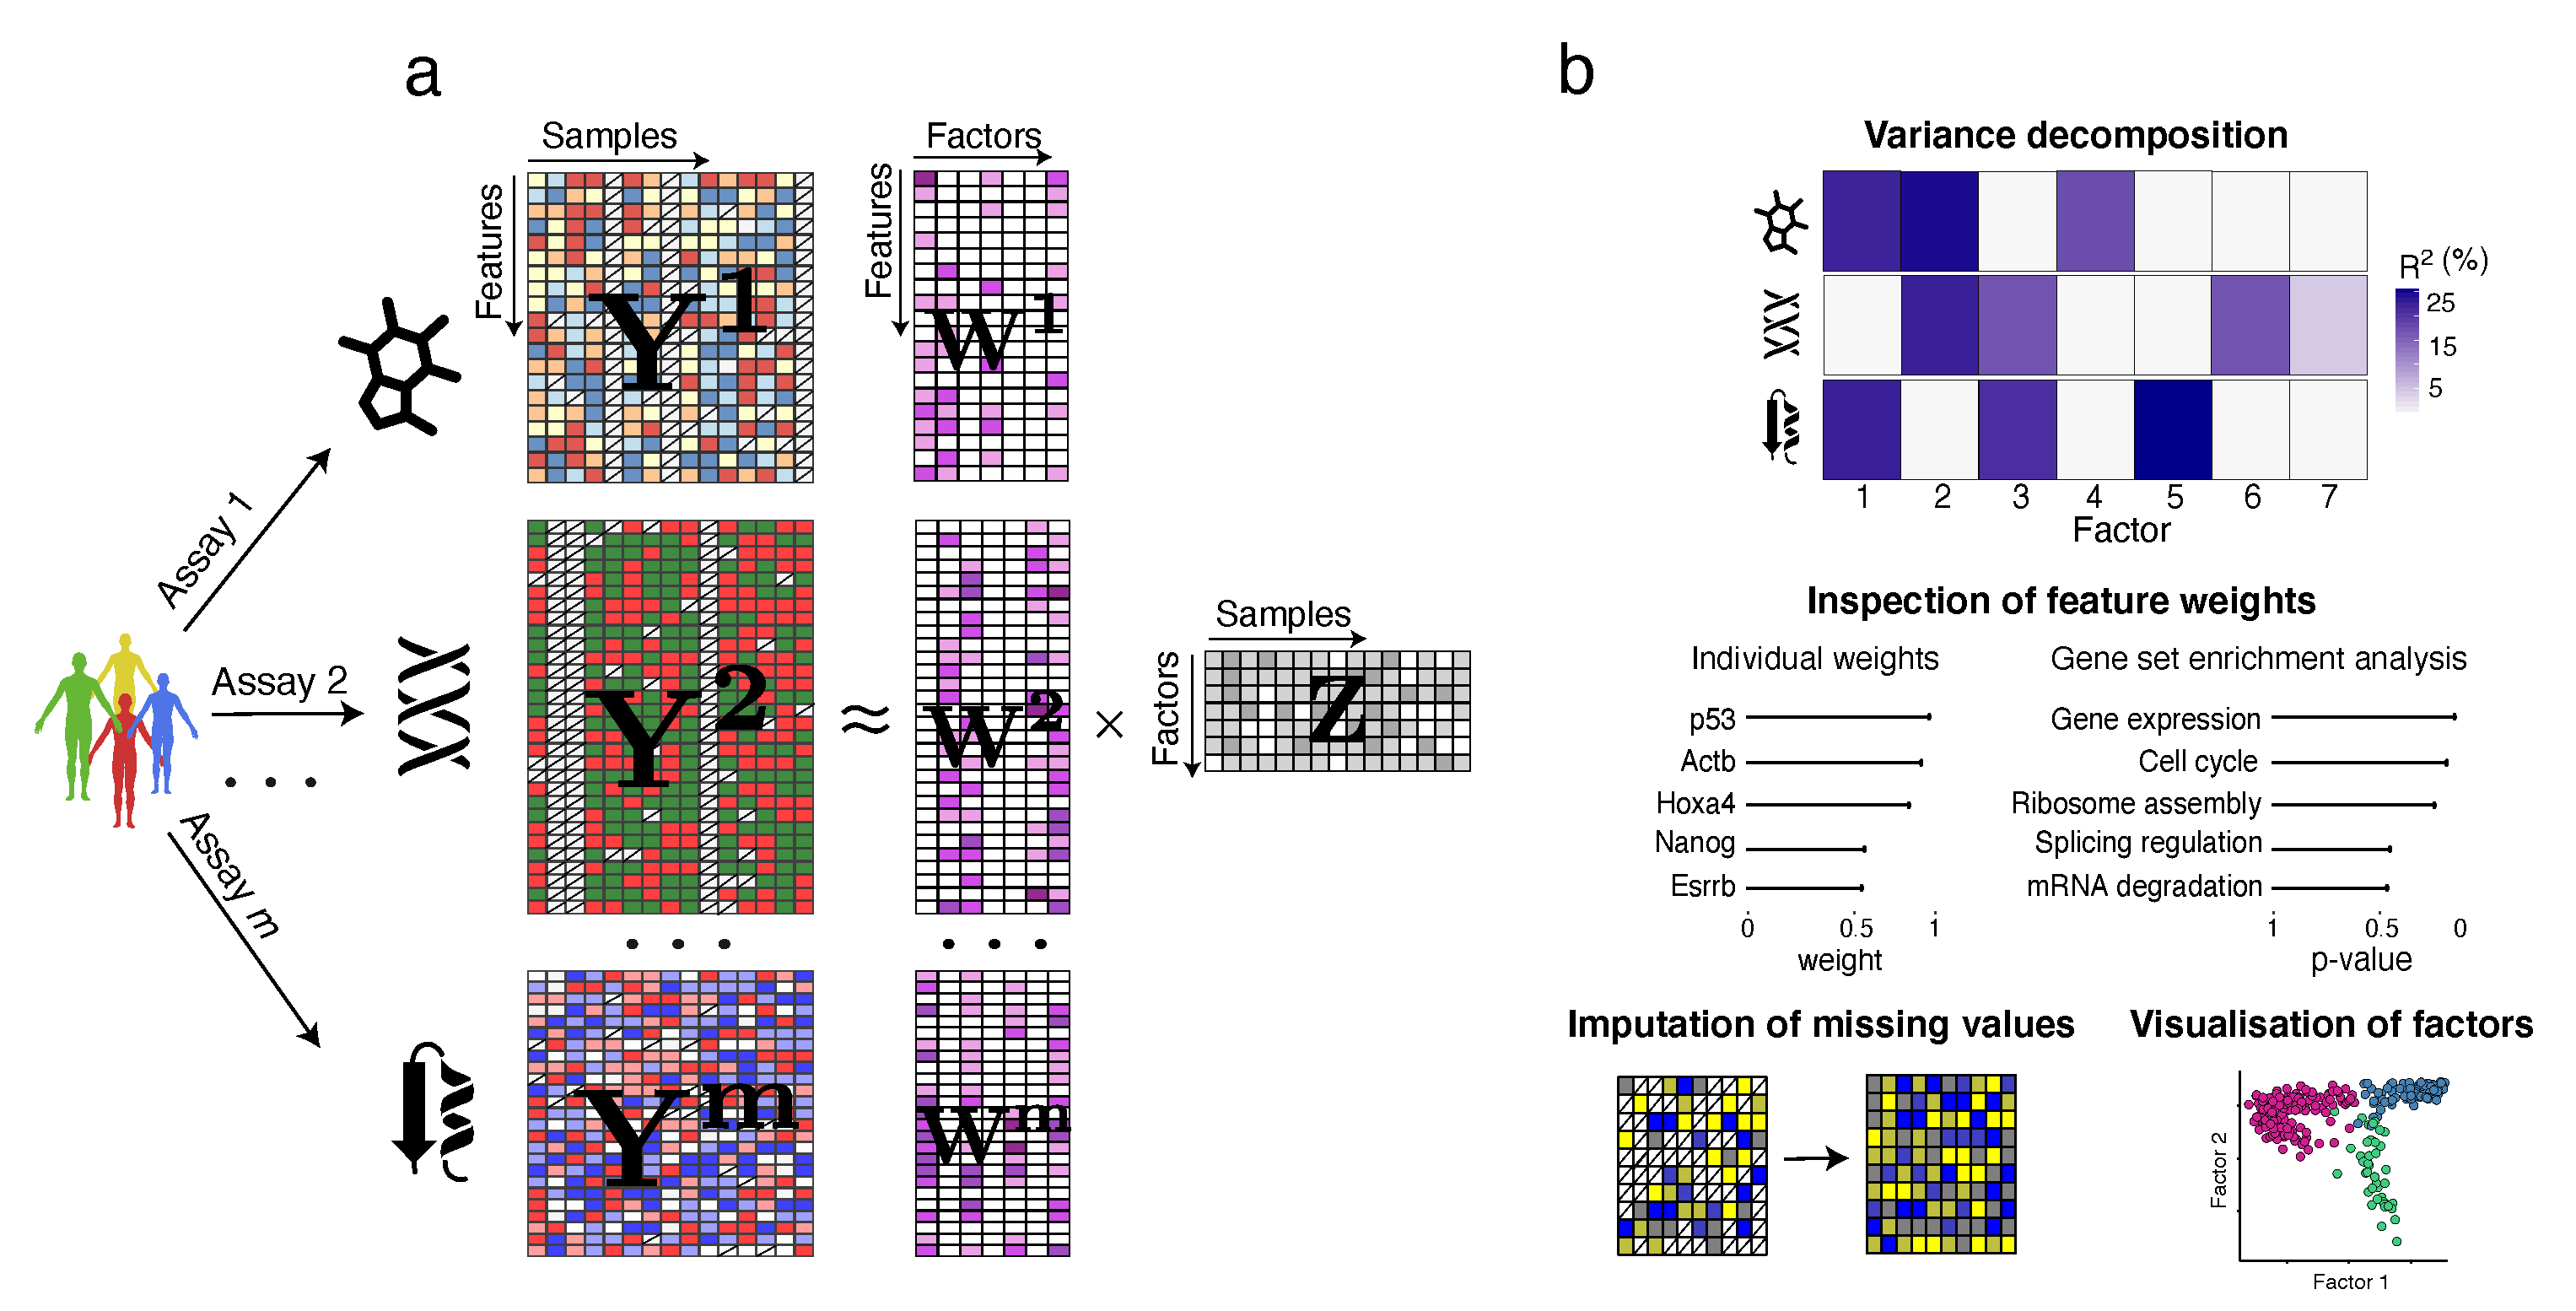
\includegraphics[width=1.0\textwidth]{MOFA}
		\caption{MOFA overview. The model takes $M$ data matrices as input ($\bfY^1, \cdots, \bfY^M$), one or more from each data modality, with co-occurrent samples but features that are not necessarily related and can differ in numbers. MOFA decomposes these matrices into a matrix of factors ($\bfZ$) and $M$ weight matrices, one for each data modality ($\bfW^1, \cdots, \bfW^M$). White cells in the weight matrices correspond to zeros, i.e. inactive features, whereas the cross symbol in the data matrices denotes missing values. The fitted MOFA model can be queried for different downstream analyses, including a variance decomposition to assess the proportion of variance explained by each factor in each data modality.}
		\label{fig:MOFA}
	\end{center}
\end{figure}

\begin{figure}[H]
	\centering
	% \definecolor{colD}{rgb}{0.2, 0.2, 0.6}
\definecolor{colM}{rgb}{0.0, 0.5, 0.0}
\definecolor{colN}{rgb}{0.5, 0.0, 0.13}
\definecolor{colG}{rgb}{1.0, 0.65, 0.0}
\newcommand\op{0.25}
\colorlet{shadecolor}{black!25}

\newcommand\op{0.25}

\begin{tikzpicture}
  % Define nodes:
  % matrix factorisation level
  \node[obs]   (Y) {$y_{n,d}^m$};
  \node[latent, above=of Y, xshift=-1.5cm] (Z) {$z_{n,k}$};
  \node[latent, above=of Y, xshift=1.5cm] (W) {$w_{k,d}^m$};
  \node[latent, xshift=1.5cm] (Tau) {$\tau_{d}^m$};

  % \node[opacity=\op,latent, xshift=-1.5cm] (Tau2) {$\tau_{n}$};

  % parents of Z
  \node[opacity=\op, det, above=of Z] (crossZ) {$\times$};
  \node[opacity=\op, latent, above=of crossZ] (Zhat) {$\hat{z}_{n,k}^{\ }$};
  \node[opacity=\op, latent, above=of Zhat] (SigmaZ) {$\alpha_k$};
  \node[opacity=\op, latent, above=of crossZ, xshift=-1.5cm] (SZ) {$s_{n,k}$};
  \node[opacity=\op, latent, above=of SZ] (ThetaZ) {$\theta_{k}$};

  % parents of W
  \node[det, above=of W] (crossW) {$\times$};
  \node[latent, above=of crossW] (What) {$\hat{w}_{k,d}^m$};
  \node[latent, above=of What] (SigmaW) {$\alpha_k^m$};
  \node[latent, above=of crossW, xshift=1.5cm] (SW) {$s_{k,d}^m$};
  \node[latent, above=of SW] (ThetaW) {$\theta_{k}^m$};

  % Connect the nodes
  \edge {Z,W, Tau} {Y}; %
  \edge[opacity=\op] {ThetaZ} {SZ};
  \edge[opacity=\op] {SigmaZ} {Zhat};
  \edge {ThetaW} {SW};
  \edge {SigmaW} {What};
  % \edge[opacity=\op] {Tau2} {Y}

  \factoredge[opacity=\op] {SZ, Zhat} {crossZ} {Z};
  \factoredge {SW, What} {crossW} {W};

  % cluster plate
  % \node[latent, above=of What, xshift=-1.3cm, opacity=0.15] (muW) {$\mu^m_{k, c}$};
  % \node[latent, above=of Zhat, xshift=1.3cm, opacity=0.15] (muZ) {$\mu_{k, c}$};
  % \edge[opacity=\op] {muZ} {Zhat};
  % \edge[opacity=\op] {muW} {What};
  % \plate[] {plateC} {(muZ)(muW)} {$C$};

  % Plates
  % \plate[] {plateK} {(Z)(W)(SZ)(Zhat)(SW)(What)(ThetaZ)(ThetaW)} {$K$};
  % \plate[color=colN, fill=colN, fill opacity=0.1] {plateN} {(Y)(Z)(crossZ)(Zhat)(SZ)(plateK.south west)} {\color{colN} $N$};
  % \plate[color=colD ,fill=colD, fill opacity=0.1] {plateD} {(Y)(W)(Tau)(crossW)(What)(SW)(plateK.south east) (plateN.south east)} {\color{colD}$D_m$};
  % \plate[color=colM,fill=colM, fill opacity=0.1] {plateM} {(plateD)(ThetaW)(plateK.north east)} {\color{colM}$M$};
  \plate[] {plateK} {(Z)(W)(SZ)(Zhat)(SW)(What)(ThetaZ)(ThetaW)} {$K$};
  \plate[] {plateN} {(Y)(Z)(crossZ)(Zhat)(SZ)(plateK.south west)} {$N$};
  \plate[] {plateD} {(Y)(W)(Tau)(crossW)(What)(SW)(plateK.south east) (plateN.south east)} {$D_m$};
  \plate[] {plateM} {(plateD)(ThetaW)(plateK.north east)} {$M$};

\end{tikzpicture}

	\caption{Graphical model for MOFA. The white circles represent hidden variables that are infered by the model, whereas the grey circles represent the observed variables. There are a total of four plates, each one representing a dimension of the model: $M$ for the number of views, $N$ for the number of samples, $K$ for the number of factors and $D_m$ for the number of features in the $m$-th view. The use of transparency in the top left nodes is intentional and becomes clear in Chapter 4 where we implement a spike-and-slab prior on the factors.}
	\label{fig:MOFA_graphical_model}
\end{figure}

\subsubsection{Inference}
To make the model scalable to large data sets we adopt a Variational inference framework with a structured mean field approximation. A detailed overview is given in \Cref{section:variational_inference}, and details on the variational updates for the MOFA model are given in \Cref{Appendix XX}. To enable efficient inference for non-Gaussian likelihoods we employ local bounds \cite{Jaakkola2000,Seeger2012}. This is described in detail in \Cref{section:mofa_ngaussian}


\subsection{Model selection and consistency across random initilizations} \label{section:mofa_robustness}
The optimisation problem in MOFA is not convex and the resulting posterior distributions depend on the initialisation of the model. Thus, when doing random initialisation of the parameters and/or expectations it becomes mandatory to perform model selection and assess the consistency of the factors across different trials.\\
The strategy we adopted in this work is to train several instances MOFA models under different parameter initialisations, where the expectation of each node is randomly sampled from its underlying distribution. After fitting, we select the model with the highest ELBO for downstream analysis. In addition, we evaluate the robustness of the factors by plotting the Pearson correlations between factors across all trials:

\begin{figure}[H]
	\centering 	
	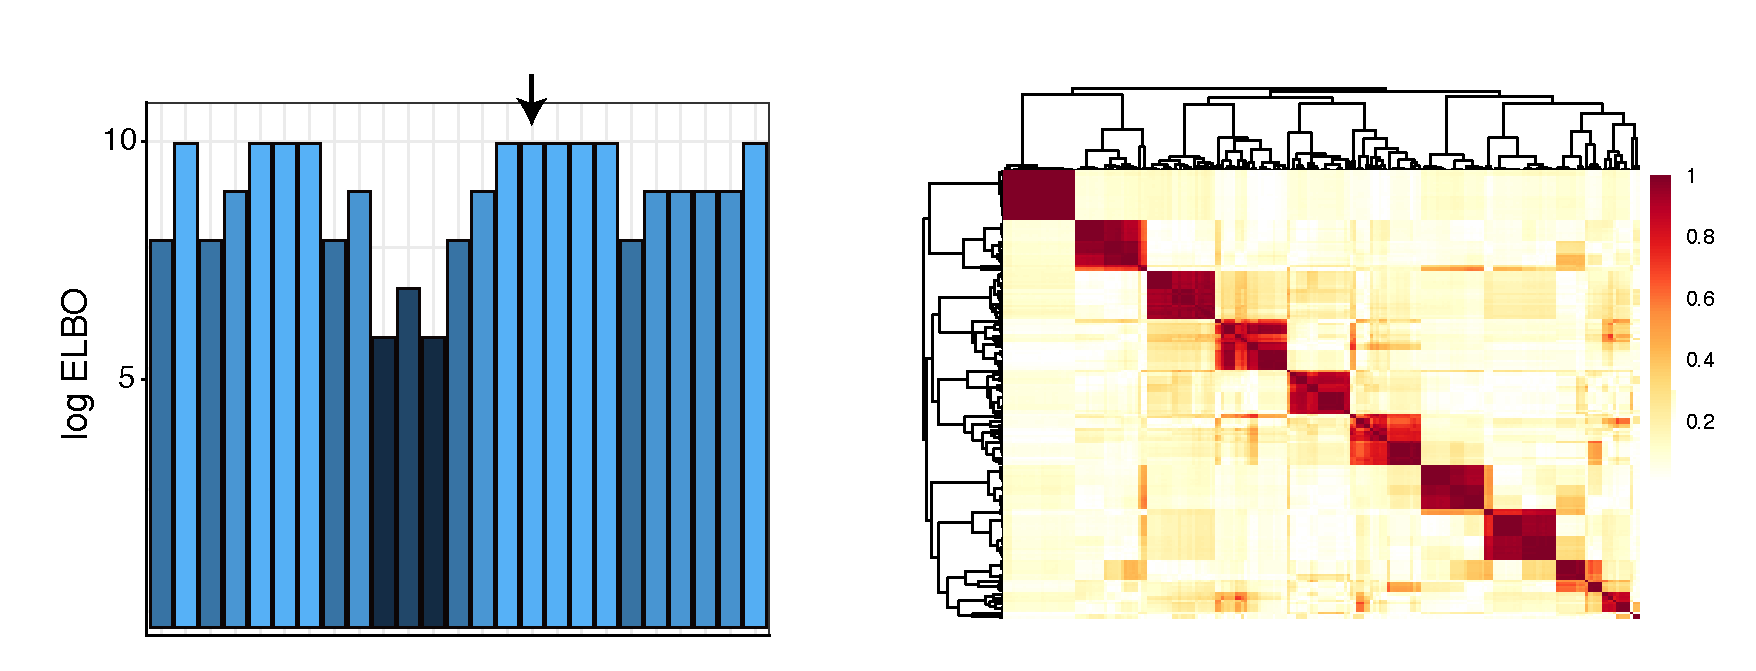
\includegraphics[width=1.0\textwidth]{MOFA_robustness}
	\caption{ \textbf{Model selection and robustness analysis in MOFA}.\\
	The left plot the log ELBO (y-axis) for 25 model instances (x-axis). The arrow indicates the model with the highest ELBO that would be selected for downstream analysis. The right plot displays the absolute value of the Pearson correlation coefficient between pairwise combinations of all factors across the 25 model instances. A block-diagonal matrix indicates that factors are robustly estimated regardless of the initialisation.}
	\label{fig:MOFA_robustness}
\end{figure}

\subsection{Learning the number of factors} \label{section:mofa_nfactors}
As described in \Cref{ard}, the use of an ARD prior allows factors to be actively prunned by the model if their variance explained is negligible. In the implementation we control the prunning of factors by a hyperparameter that defines a threshold on the minimum fraction of variance explained by a factor (across all views).\\
Additionally, because of the non-convexity of the optimisation problem, different model instances can potentially yield solutions with different number of active factors (\Cref{fig:mofa_nfactors}). Thus, the optimal number of factors can be selected by the model selection strategy outlined in \Cref{section:mofa_robustness}.

\begin{figure}[H]
	\centering 	
	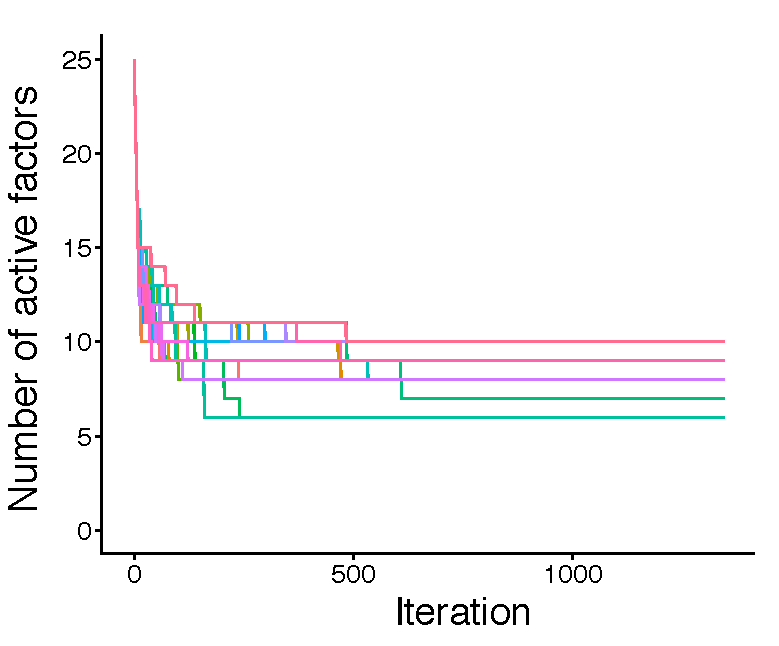
\includegraphics[width=0.5\textwidth]{MOFA_nfactors}
	\caption{\textbf{Training curve for the number of active factors across 25 different model instances}.\\
	The y-axis displays the number of active factors. The x-axis displays the iteration number. Different lines denote different model instances.}
	\label{fig:mofa_nfactors}
\end{figure}

\subsection{Monitoring convergence}
An attractive property ofvVariational inference is that the objective function, the Evidence Lower Bound (ELBO), increases monotonically at every iteration. This provides a simple way of monitoring convergence:

 \begin{figure}[H]
	\centering 	
	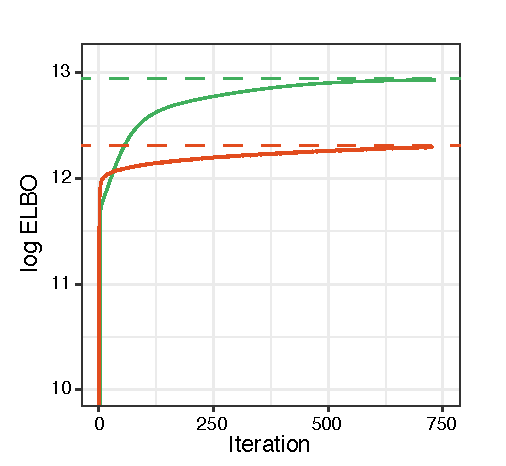
\includegraphics[width=0.5\textwidth]{elbo_convergence}
	\caption{Training curve for two diffent initialisations of MOFA. The y-axis displays the log of the ELBO, with higher values indicating a better fit. The x-axis displays the iteration number. The horizontal dash lines mark the value of the ELBO upon convergence. }
	\label{fig:elbo_convergence}
\end{figure}

Training is stopped when the change in the lower bound becomes smaller than a predefined threshold. In MOFA we implemented

\subsection{Modelling and inference with non-Gaussian data} \label{section:mofa_ngaussian}
To implement efficient variational inference in conjunction with a non-Gaussian likelihood we adapt prior work from \cite{Seeger2012} using local variational bounds. The key idea is to dynamically approximate non-Gaussian data by Gaussian pseudo-data based on a second-order Taylor expansion.  To make the approximation justifiable we need to introduce variational parameters that are adjusted alongside the updates to improve the fit.	\\
Denoting the parameters in the MOFA model as $\bfX= (\bfZ,\bfW,\balpha,\btau,\btheta)$, recall that the variational framework approximates the posterior $p(\bfX | \bfY )$ with a distribution $q(\bfX)$, which is indirectly optimised by optimising a lower bound of the log model evidence. The resulting optimization problem can be re-written as
\begin{equation*}
\min_{q(\bfX)} -\Lagr(\bfX) =  \min_{q(\bfX)} \E_q \big[ -\log p(\bfY|\bfX) \big] + \KL[q(\bfX)||p(\bfX)].
\end{equation*}


Expanding the MOFA model to non-Gaussian likelihoods we now assume a general likelihood of the form $p(\bfY|\bfX)=p(\bfY|\bfC)$ with $\bfC = \bfZ\bfW^{T}$, that can write as

\begin{equation*}
-\log p(\bfY|\bfX) = \sum_{n=1}^{N} \sum_{d=1}^{D} f_{nd} (c_{nd})
\end{equation*}
with $f_{nd}(c_{nd}) = -\log p(y_{nd}|c_{nd})$. We dropped the view index $m$ to keep notation uncluttered.\\
Extending \cite{Seeger2012} to our heteroscedastic noise model, we require $f_{nd}(c_{nd})$ to be twice differentiable and bounded by $\kappa_d$, such that $f_{nd}''(c_{nd}) \leq \kappa_d \,\forall n,d$. This holds true in many important models as for example the Bernoulli and Poisson case. Under this assumption a lower bound on the log likelihood can be constructed using Taylor expansion,
\begin{equation*}
f_{nd}(c_{nd}) \leq \frac{\kappa_d}{2} (c_{nd} - \zeta_{nd})^2 + f'(\zeta_{nd})(c_{nd} - \zeta_{nd}) + f_{nd}(\zeta_{nd}) := q_{nd}(c_{nd},\zeta_{nd}),
\end{equation*}
where $\bZeta =  \zeta_{nd} $ are additional variational parameters that determine the location of the Taylor expansion and have to be optimised to make the lower bound as tight as possible. Plugging the bounds into above optimization problem, we obtain:
\begin{equation*}
\min_{q(\bfX),\bZeta} \quad \sum_{d=1}^{D}\sum_{n=1}^{N} \E_q [ q_{nd}(c_{nd},\zeta_{nd})] + \KL[q(\bfX)||p(\bfX)]
\end{equation*}
The algorithm propsed in \cite{Seeger2012} then alternates between updates of $\bZeta$ and $\mathrm{q}(\bTheta)$. The update for $\bZeta$ is given by
\begin{equation*}
\zeta \leftarrow \E[\bfW]\E[\bfZ]^{T}
\end{equation*}
where the expctations are taken with respect to the corresponding $q$ distributions.\\
% In order to find the updates for $q(\bTheta)$ we bring the taylor approximation of $q(f_{nd})$ in q audratic form:
% \begin{equation*}
% q(f_{nd},\zeta_{nd}) \propto \frac{\kappa_d}{2}(f_{nd} - (zeta_{nd} - g(\zeta_{nd})/\kappa_d))^2
% \end{equation*}
% and note that this is proportional to the log of a Gaussian distribution $-log \Normal (\hat{y}_{nd}|f_{ng},\frac{1}{ng})$ where $\hat{y}_{nd} = zeta_{nd} - g'(\zeta_{nd})/\kappa_d$ is defined as a pseudodata based on the zero-inflated observations.
% Consequently, for fixed $\zeta_{nd}$, the updates of the variational distributions $Q(X)$ and $Q(W)$ are equivalent to the ones derived in X, but with pseudodata $\hat{Y}$ and precision $\kappa_g$
On the other hand, the updates for $q(\bfX)$ can be shown to be identical to the variational Bayesian updates with a conjugate Gaussian likelihood when replacing the observed data $\bfY$ by a pseudo-data $\hat{\bfY}$ and the precisions $\tau_{nd}$ (which were treated as random variables) by the constant terms $\kappa_d$ introduced above.\\
The pseudodata is given by
\begin{equation*}
\hat{y}_{nd} = \zeta_{nd} - f'(\zeta_{nd})/\kappa_d.
\end{equation*}
Depending on the log likelihoods $f(\cdot)$ different $\kappa_d$ are used resulting in different pseudo-data updates. Two special cases implemented in MOFA are the Poisson and Bernoulli likelihood described in the following.

\subsubsection*{Bernoulli likelihood for binary data}
When the observations are binary, $y \in \{0,1\}$, they can be modelled using a Bernoulli likelihood:
%\begin{equation*}
%p(y|c) = \frac{e^{yc}}{1+e^c}
%\end{equation*}
%The second derivative of the log likelihood is bounded by:
%\begin{equation*}
%f''(c) = \sigma(c)\sigma(-c) \leq 1/4 := \kappa
%\end{equation*}
%where $\sigma$ is the sigmoid function $f(c) = 1/(1+e^{-c})$.\\
%The pseudodata updates are given by
%\begin{equation*}
%\hat{y}_{nd} = \zeta_{nd} - 4*(\sigma(\zeta_{nd}) - y_{nd})
%\end{equation*}
\begin{equation*}
\bfY|\bfZ,\bfW \sim \text{Ber}(\sigma(\bfZ\bfW^T)),
\end{equation*} where $\sigma(a)=(1+e^{-a})^{-1}$ is the logistic link function and $\bfZ$ and $\bfW$ are the latent factors and weights in our model, respectively.\\
In order to make the variational  inference efficient and explicit as in the Gaussian case, we aim to approximate the Bernoulli data by a Gaussian pseudo-data as proposed in \cite{Seeger2012} and described above which allows to recycle all the updates from the model with Gaussian views. While \cite{Seeger2012} assumes a homoscedastic approximation with a spherical Gaussian, we adopt an approach following \cite{Jaakkola2000}, which allows for heteroscedaticity and provides a tighter bound on the Bernoulli likelihood.\\
Denoting $c_{nd}=(\bfZ\bfW^T)_{nd}$ the Jaakkola upper bound \cite{Jaakkola2000} on the negative log-likelihood is given by
\begin{align*}
\begin{split}
-\log\left(p(y_{nd}|c_{nd})\right) &= -\log\left(\sigma\left((2y_{nd}-1)  c_{nd}\right)\right)\\
& \leq -\log(\zeta_{nd})-\frac{(2y_{nd}-1)c_{nd}-\zeta_{nd})}{2} +\lambda(\zeta_{nd})\left(c_{nd}^2 -\zeta_{nd}^2 \right)\\
& =: b_J(\zeta_{nd}, c_{nd},y_{nd} )
\label{jaakkola}
\end{split}
\end{align*}
with $\lambda$ given by $\lambda(\zeta)=\frac{1}{4\zeta}\tanh\left(\frac{\zeta}{2}\right)$.\\
This can easily be derived from a first-order Taylor expansion on the function $f(x) = - \log(e^{\frac{x}{2}}+e^{-\frac{x}{2}}) = \frac{x}{2}-\log(\sigma(x))$ in $x^2$ and by the convexity of 
$f$ in $x^2$ this bound is global as discussed in \cite{Jaakkola2000}.\\
In order to make use of this tighter bound but still be able to re-use the variational updates from the Gaussian case we re-formulate the bound as a Gaussian likelihood on pseudo-data $\hat{\bfY}$.\\
As above we can plug this bound on the negative log-likelihood into the variational optimization problem to obtain  \begin{equation*}
\min_{q(\bfX),\bZeta} \quad \sum_{d=1}^{D}\sum_{n=1}^{N} \mathbb{E}_q b_J(\zeta_{nd}, c_{nd},y_{nd} ) + \KL[q(\bfX)||p(\bfX)].
\end{equation*}
This is minimized iteratively in the variational parameter $\zeta_{nd}$ and the variational distribution of Z,W:\\
Minimizing in the variational parameter $\zeta$ this leads to the updates given by
\begin{equation*}
\zeta_{nd}^2 = \mathbb{E}[c_{nd}^2]
\end{equation*}
as described in \cite{Jaakkola2000}, \cite{Bishop}.\\
For the variational distribution $q(\bfZ,\bfW)$ we observe that the Jaakkola bound can be re-written as 
\begin{equation*}
b_J(\zeta_{nd}, c_{nd},y_{nd} ) = -\log\left(\varphi\left(\hat{y}_{nd}; c_{nd}, \frac{1}{2\lambda(\zeta_{nd})}\right)\right) + \gamma(\zeta_{nd}),
\end{equation*}
where $\varphi(\cdot; \mu, \sigma^2)$ denotes the density function of a normal distribution with mean $\mu$ and variance $\sigma^2$ and $\gamma$ is a term only depending on $\bZeta$. This allows us to re-use the updates for $\bfZ$ and $\bfW$ from a setting with Gaussian likelihood by considering the Gaussian pseudo-data 
\begin{equation*}
\hat{y}_{nd}= \frac{2y_{nd}-1}{4 \lambda(\zeta_{nd})}
\end{equation*}
updating the data precision as $\tau_{nd} = 2\lambda(\zeta_{nd})$ using  updates generalized for sample- and feature-wise precision parameters on the data.


\subsubsection*{Poisson likelihood for count data}
When observations are a natural numbers, such as count data $y \in \N = \{0,1,\cdots\}$, they can be modelled using a Poisson likelihood:
\begin{equation*}
p(y|c) = \lambda(c)^y e^{-\lambda(c)}
\end{equation*}
where $\lambda(c)>0$ is the rate function and has to be convex and log-concave in order to ensure that the likelihood is log-concave.\\
As done in \cite{Seeger2012}, here we choose the following rate function: $\lambda(c)=\log(1+e^c)$.

Then an upper bound of the second derivative of the log-likelihood is given by
\begin{equation*}
f''_{nd}(c_{nd}) \leq \kappa_d = 1/4 + 0.17*\max(\bfy_{:,d}).
\end{equation*}
%The bound degrades with the presence of entries with large values. Thus, we follow common practice and clip overly large counts.\\
The pseudodata updates are given by
\begin{equation*}
\hat{y}_{nd} = \zeta_{nd} - \frac{\mathrm{S}(\zeta_{nd})(1-y_{nd}/\lambda(\zeta_{nd}))}{\kappa_d}.
\end{equation*}


\newpage


\subsection{Model validation with simulated data} \label{section:mofa_simulated}
We used simulated data from the generative model to systematically test the technical capabilities of MOFA.

\subsubsection{Recovery of simulated factors}
First, we tested the ability of MOFA to recover simulated factors under varying number of views, features, factors and with different amounts of missing values.\\ 
For every simulation scenario we initialised a model with a high number of factors ($K=100$), and inactive factors were automatically dropped during model training by the ARD prior. In addition, to test the robustness under different random initialisations, ten model instances were trained for every simulation scenario.\\
We observe that in most settings the model accurately recovers the correct number of factors (\Cref{fig:MOFA_learnK}). Exceptions occur when the dimensionality of the latent space is too large (more than 50 factors) or when an excessive amount of missing values (more than 80\%) is present in the data.

\begin{figure}[H]
	\centering 	
	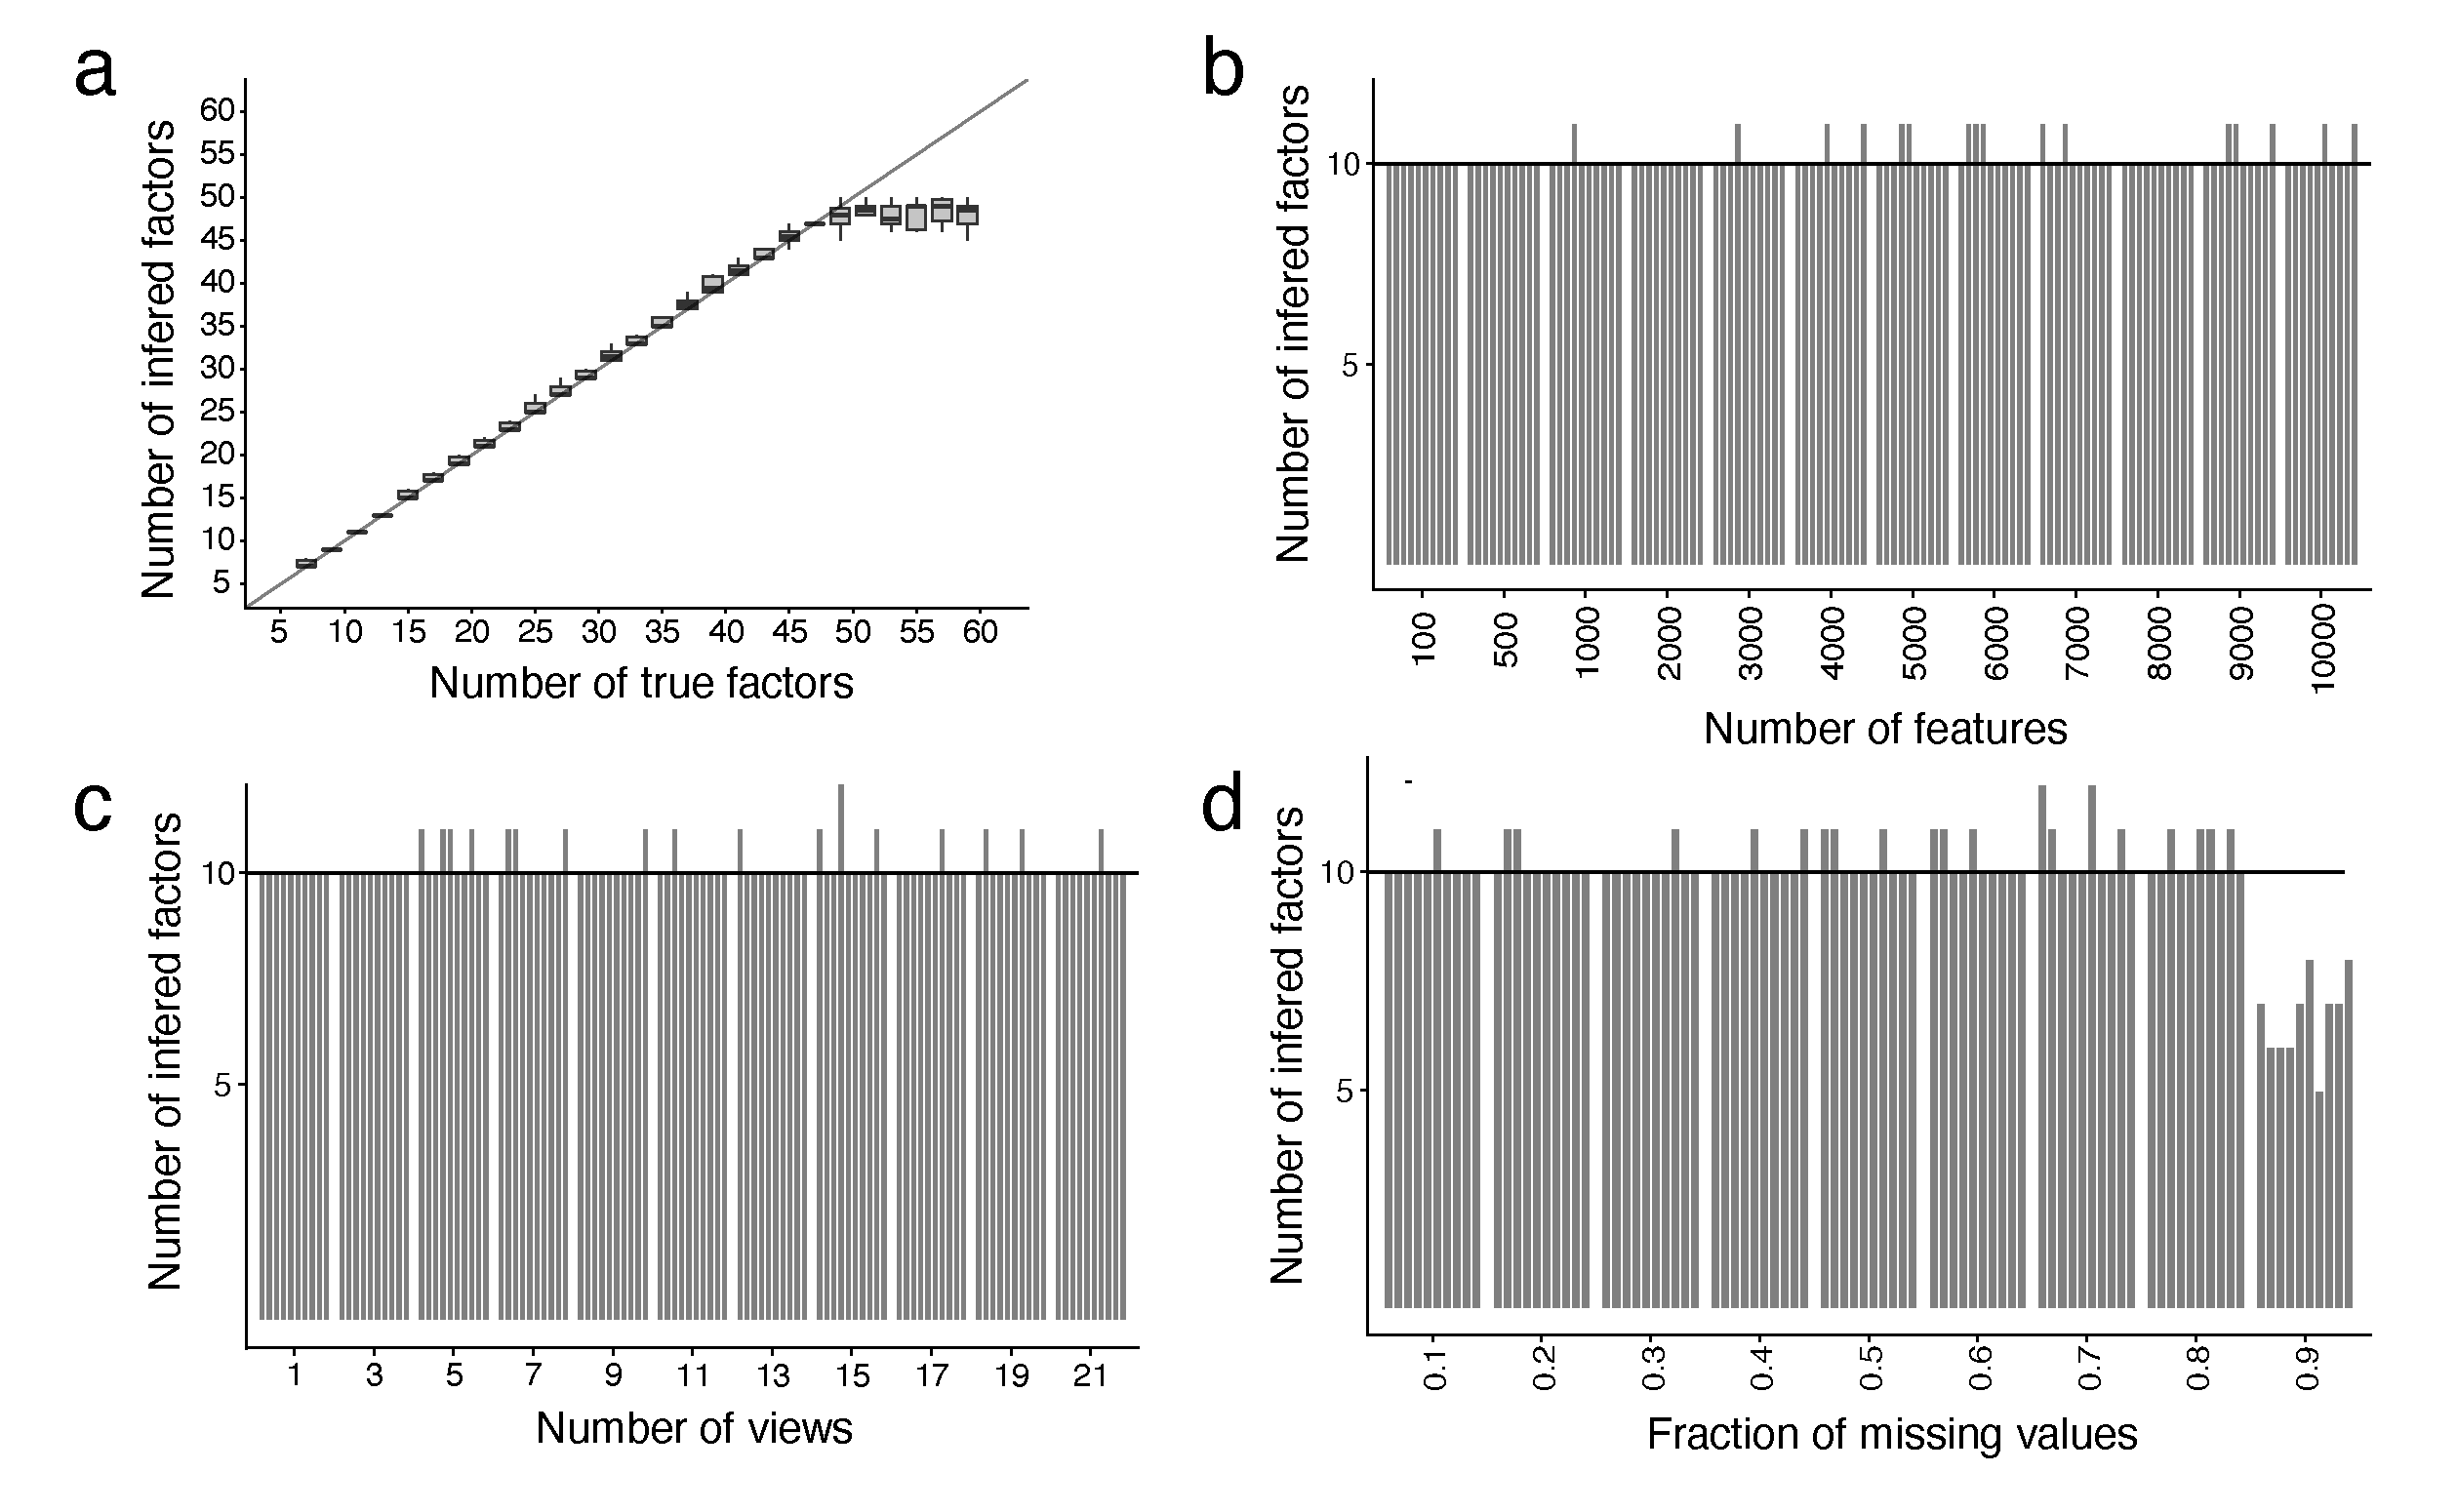
\includegraphics[width=1.0\textwidth]{MOFA_learnK}
	\caption{\textbf{Assessing the ability to recover simulated factors}.\\
	In all plots the y-axis displays the number of infered factors. (a) x-axis displays the number of true factors, and boxplots summarise the distribution across 10 model instances. For (c-d) the true number of factors was set to $K=10$ and each bar corresponds to a different model instance. (b) x-axis displays the number of features, (c) x-axis displays the number of views, (d) x-axis displays fraction of missing values. }
	\label{fig:MOFA_learnK}
\end{figure}

\subsubsection{View-wise sparsity on the weights}
One of the most important statistical assumptions underlying MOFA is the ARD prior aimed at disentangling the activity of factors across views (see \Cref{section_ard} and \Cref{mofa:model_description}.\\
We simulated data from the generative model were the factors were set to be active or inactive in specific views by sampling $\alpha_{k}^{m}$ from a discrete distribution with values $\{ 1, 1e3\}$. We compared the performance with a popular integrative clustering method (iCluster) that is also formulated as a latent variable model \cite{Mo2013}. In iCluster each factor shares the same sparsity constraint across all views, and hence the model is less accurate when it comes to the detection of factors that show differential activity across different views.:

\begin{figure}[H]
	\centering 	
	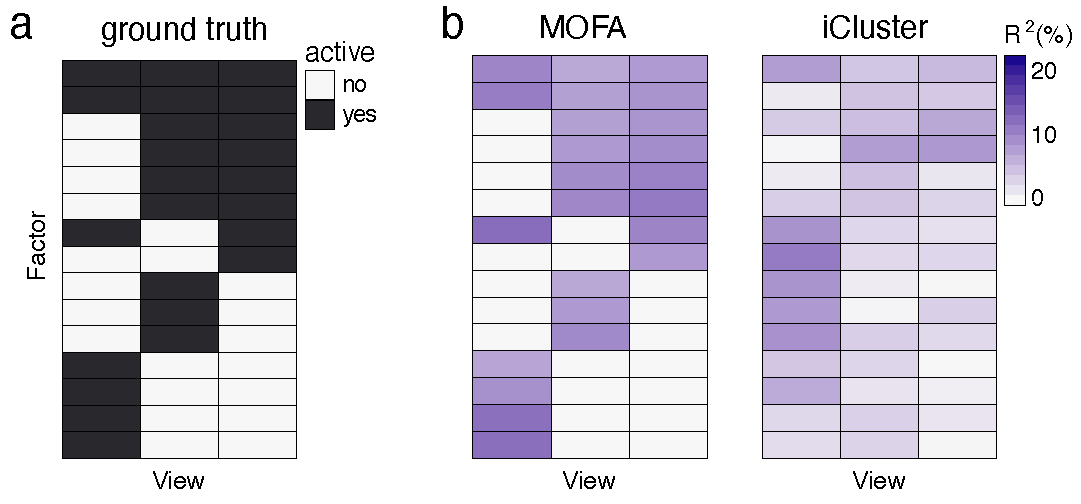
\includegraphics[width=1.0\textwidth]{MOFA_group_sparsity}
	\caption{\textbf{Evaluating the ability to recover differential factor activity across views}.\\
	(a) The true activity pattern, with factors sampled to display differential activity across views.
	(b) Percentage of variance explained for each factor in each view, for MOFA and iCluster\cite{Mo2013}.}
	\label{fig:MOFA_group_sparsity}
\end{figure}

\subsubsection{Feature-wise sparsity on the weights} \label{section:spike_slab}
In MOFA we implemented a spike-and-slab prior prior to enforce feature-wise sparsity on the weights with the aim of delivering a more interpretable solution (see \Cref{section:mofa_weights}).\\
To assess the effect of the spike-and-slab prior we trained a group of models with and without the spike-and-slab prior. Importantly, the model without spike-and-slab priors contains the ARD prior, which should provide some degree of regularisation. To compare both options to a non-spare method, we also fit a Principal Component Analysis on the concatenated data set.\\
As expected, we observe that the spike-and-slab prior induces more zero-inflated weights, although the ARD prior provided a moderate degree of regularisation. The PCA solution was notably more dense than both bayesian models (\Cref{fig:MOFA_sparsity}).

\begin{figure}[H]
	\centering 	
	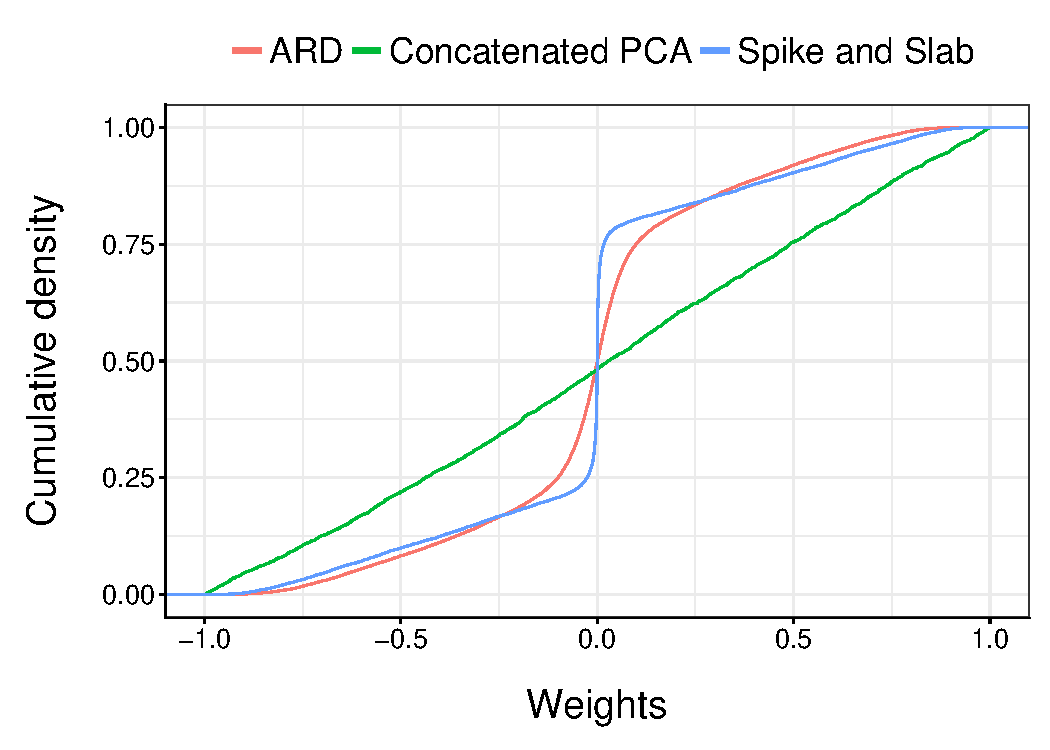
\includegraphics[width=0.7\textwidth]{MOFA_sparsity}
	\caption{\textbf{Assessing the sparsity priors on the weights}.\\ 
	The plot shows the empirical cumulative density function of the weights for an arbitrary factor in a single view. The weights were simulated with a sparsity level of $\theta_k^m=0.5$ (50\% of active features.)
	}
	\label{fig:MOFA_sparsity}
\end{figure}


\subsubsection{Non-gaussian likelihoods}  \label{section:mofa_nongaussian_results}
A key improvement of MOFA with respect to previous methods is the use of non-Gaussian likelihoods to integrate data modalities with different types of readouts. In particular, as described in \Cref{section:mofa_ngaussian}, we implemented a Bernoulli likelihood to model binary data and a Poisson likelihood to model count data.\\
To validate both likelihood models, we simulated binary and count data using the generative model and we fit two sets of models for each data type: a group of models with a Gaussian likelihood and a group of models with a Bernoulli or Poisson likelihood, respectively.\\
Reassuringly, we observe that although the Gaussian likelihood is also able to recover the true number of factors, the models with the non-Gaussian likelihoods result in a better fit to the data:

\begin{figure}[H]
	\centering 	
	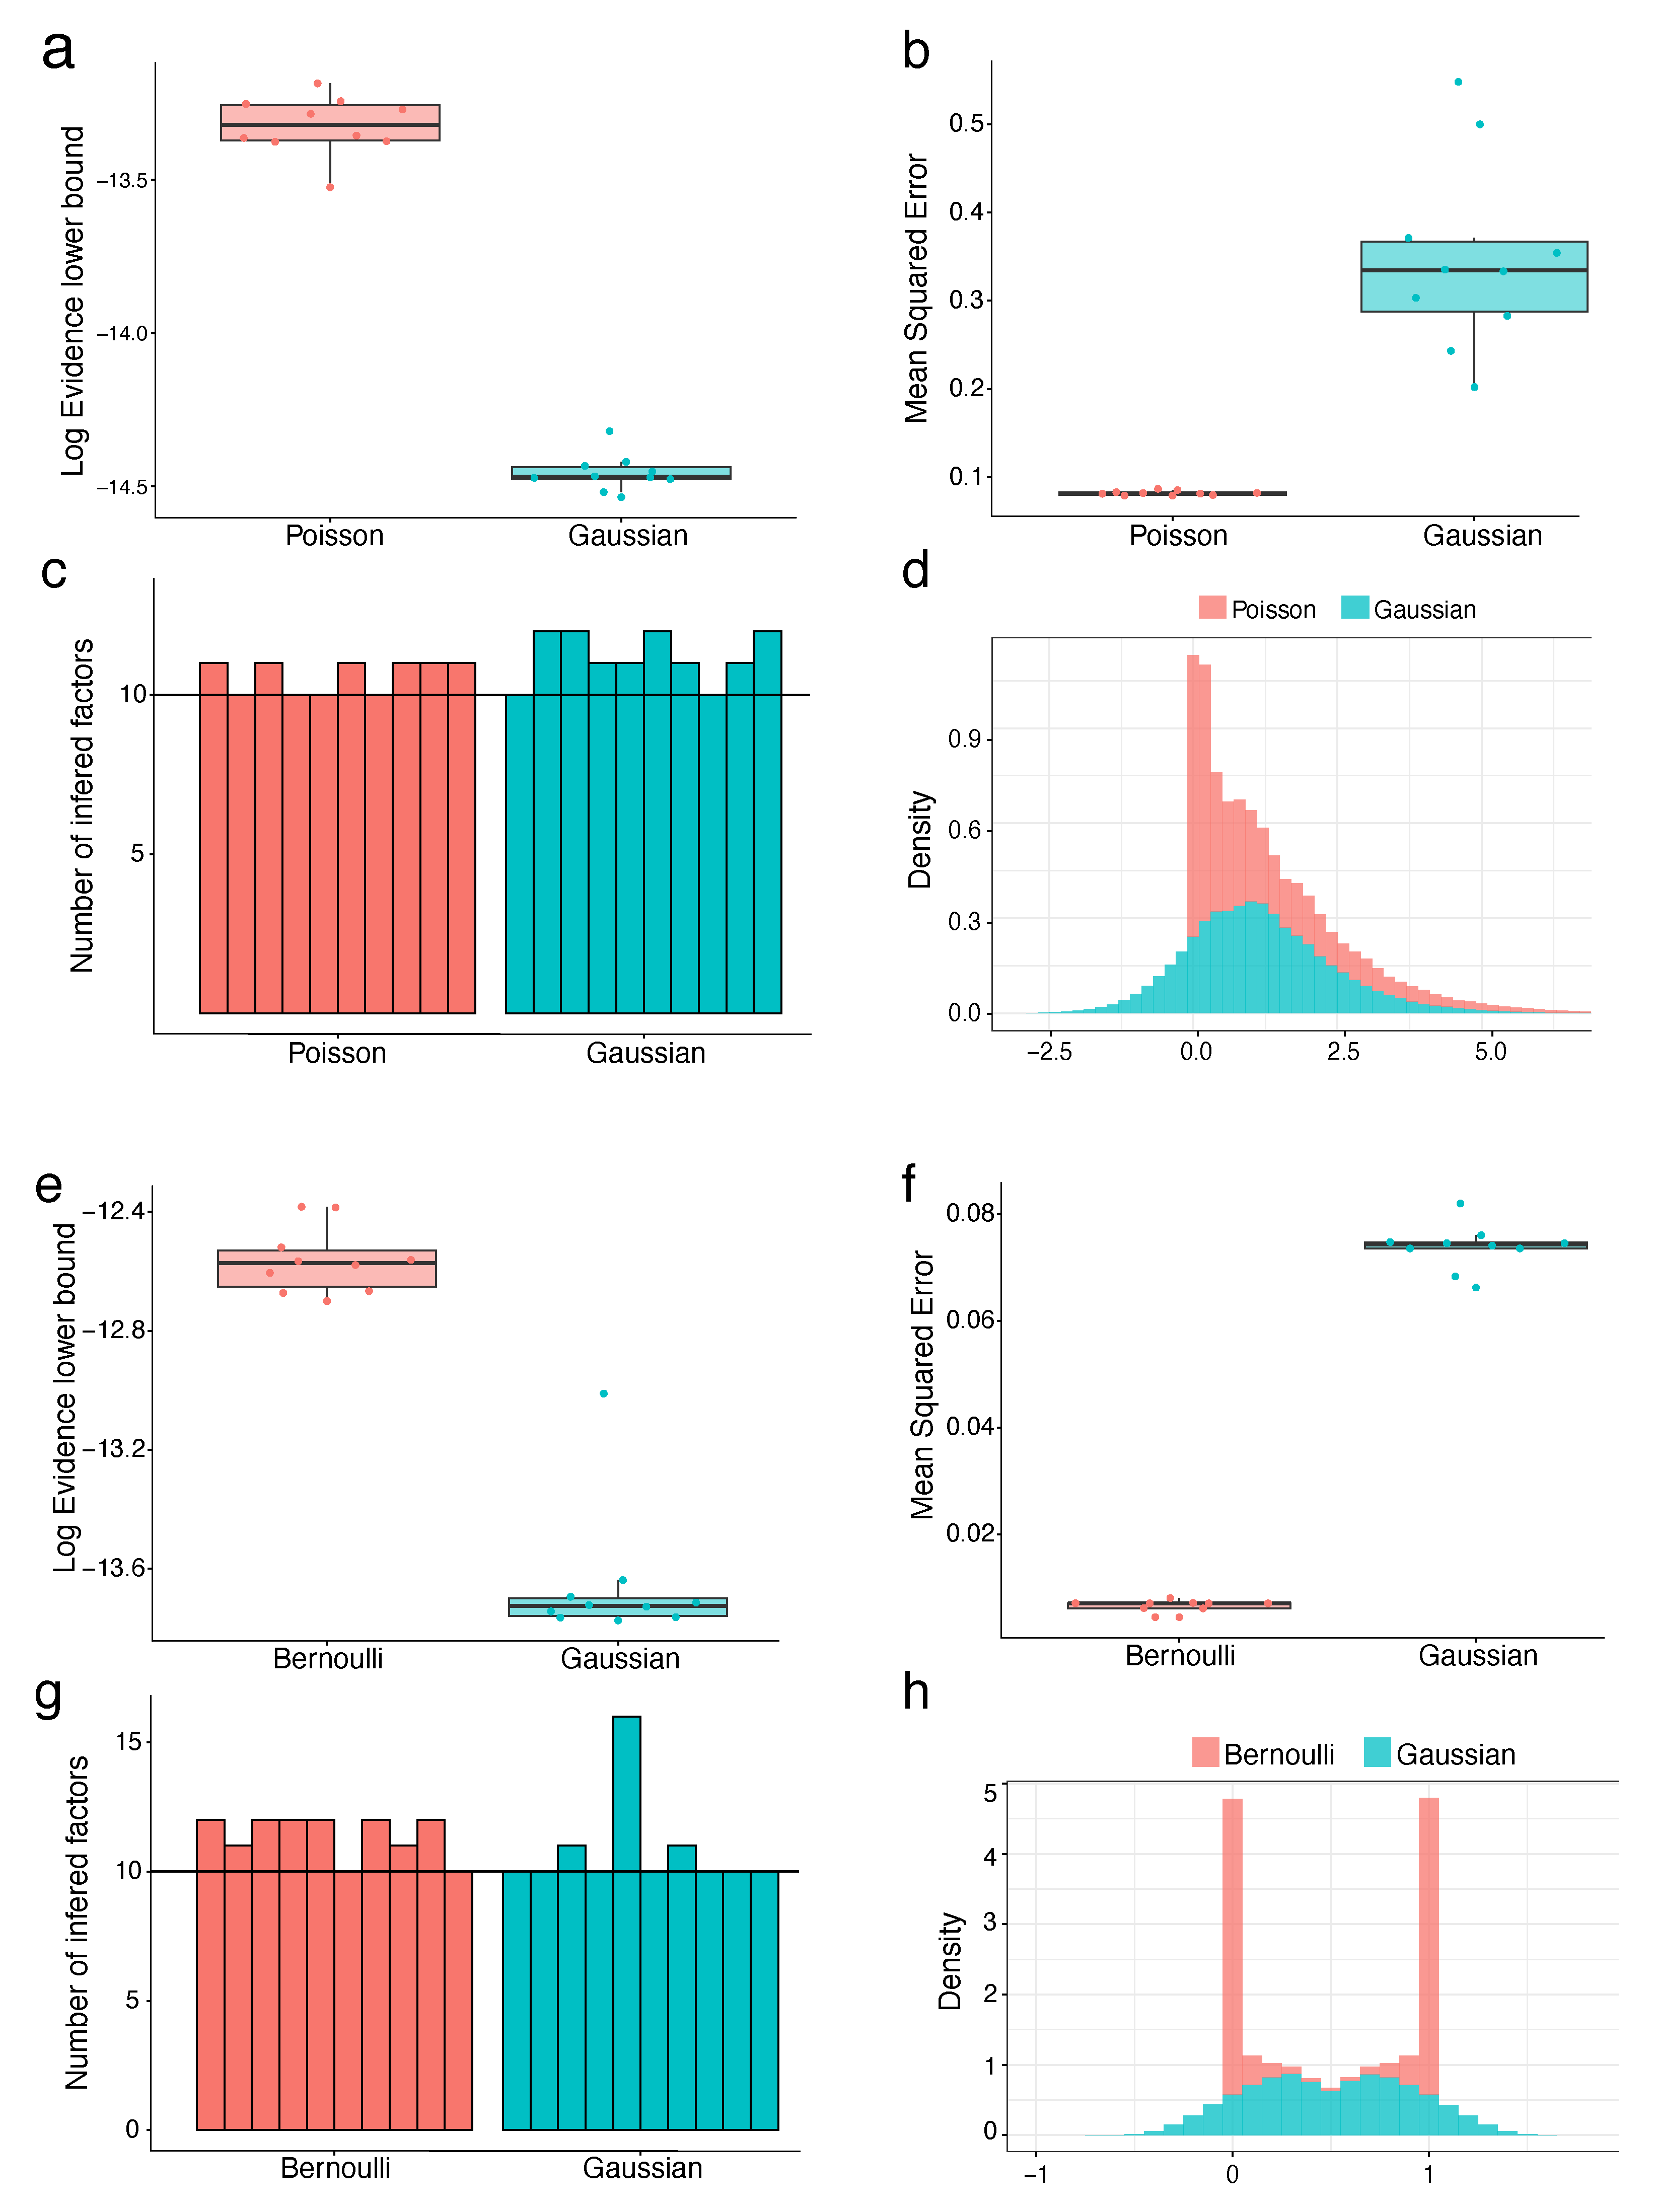
\includegraphics[width=0.9\textwidth]{MOFA_nongaussian}
	\caption{\textbf{Validation of the non-gaussian likelihood models using simulated data}.\\
	(a-d) Comparison of Poisson and Gaussian likelihood models applied to count data.\\
	(e-h) Comparison of Bernoulli and Gaussian likelihood models applied to binary data.\\
	(a,e) The y-axis displays the ELBO for each model instance (x-axis). (b,f) The y-axis displays the mean reconstruction error for each model instance (x-axis). (c,g) The y-axis displays the number of estimated factrors for each model instance (x-axis). The horizontal dashed line marks the true number of factors $K=10$. (d,h) Distribution of reconstructed data. Plotted are the expected values of the inferred posterior distributions, not samples from the corresponding posteriors. This is why reconstructed measurements are continuous and not discrete.
	}
	\label{fig:MOFA_nongaussian}
\end{figure}


% \subsubsection{Scalability}
% Finally, we evaluated the scalability of the model when varying each of its dimensions independently, and we compared the speed with a Gibbs sampling implementation of GFA \cite{Leppaaho2017} and iCluster+ \cite{Mo2013}.\\
% Overall, we observe that MOFA scales linear with respect to all dimensions and is significantly faster than any of the three evaluated techniques:
% % As a real application showcase, the training on the CLL data \Cref{fig:MOFA_CLL_Figure1} required 25 minutes using MOFA, 34 hours with GFA and 5-6 days with iCluster.

% \begin{figure}[H]
% 	\centering 	
% 	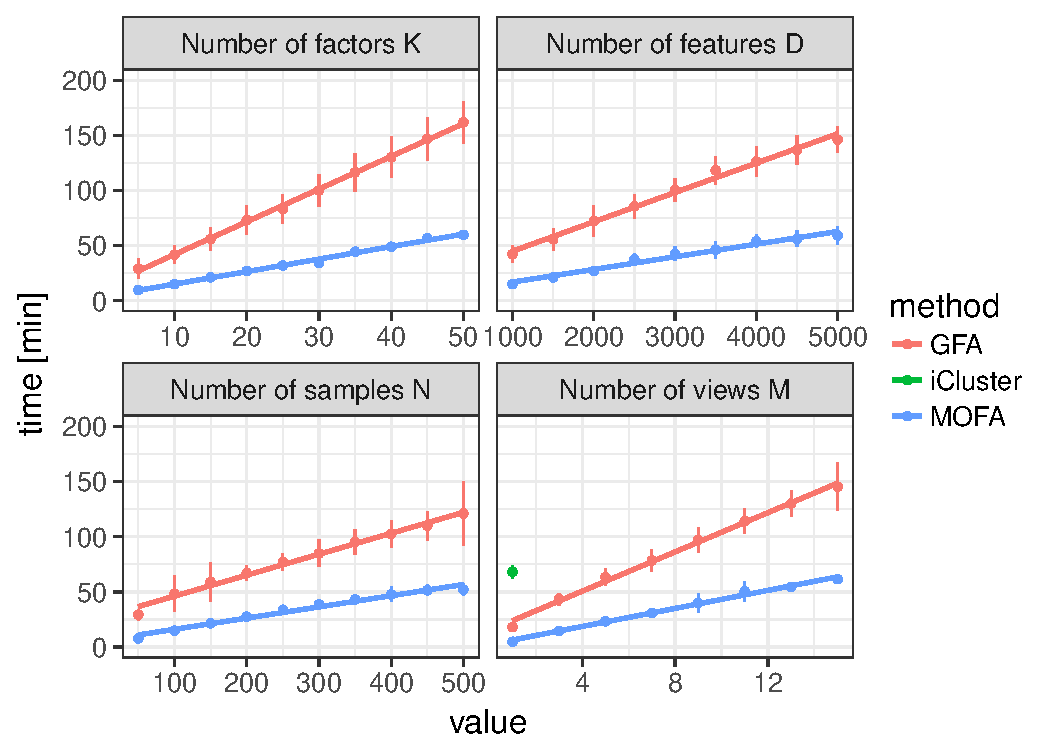
\includegraphics[width=0.9\textwidth]{MOFA_scalability}
% 	\caption{\textbf{Evaluation of speed and scalability in MOFA}.\\
% 	The y-axis displays the time required for convergence. The x-axis displays the value of the dimension that was tested, either number of factors ($K$), number of features ($D$), number of samples ($N$) and number of views ($M$). Baseline parameters were $M=3, K=10, D=1000, N=100$. Each line represents a different model, GFA (red), MOFA (blue) and iCluster (green). Default convergence criteria where used for all methods. Each dot displays the average time across 10 trials with error bars denoting the standard deviation. iCluster is only shown for one value as all other settings required more than 200min for convergence.
% 	}
% 	\label{fig:MOFA_scalability}
% \end{figure}



\subsection{Application to chronic lymphocytic leukaemia} \label{section:mofa_cll}
Personalised medicine is an attractive field for the use of multi-omics, as dissecting heterogeneity across patients is a major challenge in complex diseases, and requires data integration from multiple biological layers \cite{Chen2013,Costello2014,Alyass2015}.
%In most cases, predicting patient survival and response to a treatment is still not reliable due to a lack of predictive biomarkers and our incomplete understanding of the mechanisms underlying response heterogeneity. Identification of the main drivers of inter-patient variation and their molecular basis is an important step towards personalized treatment decisions. 

To demonstrate the potential of the method, we applied MOFA to a publicly available study of 200 patient samples of chronic lymphocytic leukaemia (CLL) profiled for somatic mutations, RNA expression, DNA methylation and \textit{ex vivo} drug responses\cite{Dietrich2018}. We selected this data set for three main reasons: (1) The complex missing data structure, with nearly 40\% samples having incomplete assays (see \Cref{fig:MOFA_CLL_Figure1}). As described in \Cref{section:mofa_missing_values}, the inference framework implemented in MOFA should cope with large amounts of missing values, including missing assays. (2) The different data modalities: after data processing, three assays had continuous observations whereas for the somatic mutations the observations were binary. As described in \Cref{section:mofa_ngaussian}, MOFA can combine different likelihood models. (3) The existence of clinical covariates: this provides an excellent test to evaluate whether the MOFA factors can capture the variation underlying clinically-relevant phenotypes.

\subsubsection{Data overview and processing}

%Data processing and normalisation is impotant for the model to work and it requires a few considerations. First, one needs to remove differences in library size between samples. If not done correctly, the signal in the data will be dominated by this (undesired) source of variation, and more subtle heterogeneity will be harder to identify. Similarly, batch effects and other undesired technical sources of variation should be regressed out \textit{a priori}.

%Second, feature selection must be performed by removing uninformative features. This is typically done by removing features with low levels across samples, followed by the selection of highly variable features. A proper feature selection will increase the signal-to-noise-ratio, it will simplify model selection and it will speed up the training procedure.

%Third, feature imbalance:

% - Feature imbalance
% - Normalisation
% - Feature selection

Here we proceed to briefly describe the different data modalities and outline the basic data processing steps that we performed before applying MOFA.

\begin{itemize}
	\item \textbf{RNA expression} was profiled using bulk RNA-seq. Genes with low counts were filtered out and the data was subsequently normalized using DESeq2 \cite{Love2014}. Feature selection was performed by considering the top 5,000 most variable genes.
	\item \textbf{DNA methylation} was profiled using Illumina 450K arrays \cite{XXX}. We converted the beta-values to M-values, as it has better statistical properties when modelled with a Gaussian distribution \cite{XXX}. Feature selection was performed by considering the top 1\% most variable CpG sites. 
	\item \textbf{\textit{Ex vivo} Drug response} was screened using the ATP-based CellTiter-Glo assay. Briefly, the asay includes a panel of 62 drugs at 5 different concentrations each, for a total of 310 measurements. 

	\item \textbf{TO FINISHSomatic mutations} were profiled using a combination of targeted and whole exome sequencing. Feature selection was performed by considering only mutations that were present in at least three samples, which resulted in a total of 69 mutations.
\end{itemize}

For more details on the data generation steps we refer the reader to \cite{Dietrich2018}.

\subsubsection{Model overview}

In this data set, MOFA recovered $K=10$ factors, each one explaining a minimum of 3\% of variance in at least one assay. Interestingly, MOFA detects Factors which are shared across several data modalities (Factors 1 and 2, sorted by variance explained). Some factors capture sources of covariation between two data modalities (Factor 3 and 5, active in the RNA expression and drug response). In addition, some factors capture variation that is unique to a single data modality (Factor 4, active in the RNA expression data).\\
All together, the 10 MOFA factors explained 41\% of variance in the drug response data, 38\% in the mRNA expression, 24\% in the DNA methylation and 24\% in somatic mutations.

\begin{figure}[H]
	\centering 	
	\includegraphics[width=1.0\textwidth]{MOFA_CLL_overview}
	\caption{\textbf{Application of MOFA to a study of chronic lymphocytic leukaemia. Model overview.}\\
	(a) Data overview. Assays are shown in different rows ($D$ = number of features) and samples ($N$) in columns, with missing samples shown using grey bars. Notice that some samples are missing entire assays.\\
	(b) Variance explained (\%) by each Factor in each assay.\\
	(c) Total variance explained (\%) for each assay by all Factors.
	}
	\label{fig:MOFA_CLL_overview}
\end{figure}

The first two Factors are the most interesting from a molecular perspective, as they capture a phenotypic effect that is manifested across all molecular layers, from the genome to the transcriptome and ultimately in the drug response assay.\\
To annotate Factors 1 and 2 we proceeded to visualise the feature weights, starting by the (binary) somatic mutation data, as it is the simplest data modality to interpret. Inspection of the top weights revealed that Factor 1 was associated with the mutation status of the immunoglobulin heavy-chain variable (IGHV) region, while Factor 2 was aligned with trisomy of chromosome 12 (\Cref{fig:MOFA_CLL_factors12}).\\
Remarkably, in a completely unsupervised fashion, MOFA recovered the two most important clinical markers in CLL as the two major axes of molecular disease heterogeneity \cite{Fabbri2016,Bulian2017,Crombie2017}.

Next, we visualised the samples in the latent space spanned by Factors 1 and 2. A scatterplot based on these factors shows a clear separation of patients by their IGHV status on the first Factor and presence or absence of trisomy 12 on the second Factor (\Cref{fig:MOFA_CLL_factors12}). Note that this latent representation enables simple patient stratification into molecular subgroups (see dashed lines), a first step towards personalised medicine.\\
Interestingly, 24 patients lacked IGHV status measurements (see grey crosses) due to quality control filtering in the DNA sequencing assay. Nonetheless, MOFA is able to pool information from the other molecular layers to map those samples to the latent space, and could be classified to the corresponding molecular subgroup.

\begin{figure}[H]
	\centering 	
	\includegraphics[width=1.0\textwidth]{MOFA_CLL_factors12}
	\caption{\textbf{Visualisation of the genetic signature underlying Factor 1 and 2}\\
	(a) Absolute loadings of the top features of Factors 1 and 2 in the Mutations data.
	(b) Visualization of samples using Factors 1 and 2. The colours denote the IGHV status of the tumours; symbol shape and colour tone indicate chromosome 12 trisomy status.
	}
	\label{fig:MOFA_CLL_factors12}
\end{figure}

IGHV status is currently the most important prognostic marker in CLL and has routinely been used to distinguish between two distinct subtypes of the disease\cite{Fabbri2016}. Molecularly, it is a surrogate of the level of activation of the B-cell receptor, which is in turn related to the differentiation state of the tumoral cells. Multiple studies have associated mutated IGHV with a better resposne to chemoimmunotherapy, whereas unmutated IGHV patients have a worse prognosis \cite{Fabbri2016,Bulian2017,Crombie2017}.\\
In clinical practice, the IGHV status has been considered binary. Our results suggest that this is a fairly good approximation, but a more complex structure with at least three groups or a potential underlying continuum (\Cref{fig:MOFA_CLL_factors12,fig:MOFA_CLL_Factor1}), as also suggested in \cite{Queiros2015}.

% \subsubsection{Detection of outlier samples}

% Interestingly, there is some discrepancy between the IGHV status predicted by MOFA and the IGHV status reported in the clinical data. Out the 200 patients, MOFA classifies 176 in accordance with the clinical label, it classifies 12 patients that lacked the clinical marker and it re-classifies 12 patients to the opposite group.\\
% To validate the MOFA-based classification, we proceeded to inspect the molecular data in more detail.

% sample-to-sample correlation matrices for the individual layers suggest that for 3 of the cases where the inferred factor disagrees with the clinical label, the molecular data supports the predicted label. The other 9 cases showed intermediate molecular sgnatures now well captured by the binary classification.
% %Based on these results, we hypothesize that a multi-omics approach based on several molecular signatures could be a more precise and robust approach to predict clinical phenotypes than the use of single features such as mutations or expression of marker genes.

% \begin{figure}[H]
% 	\centering 	
% 	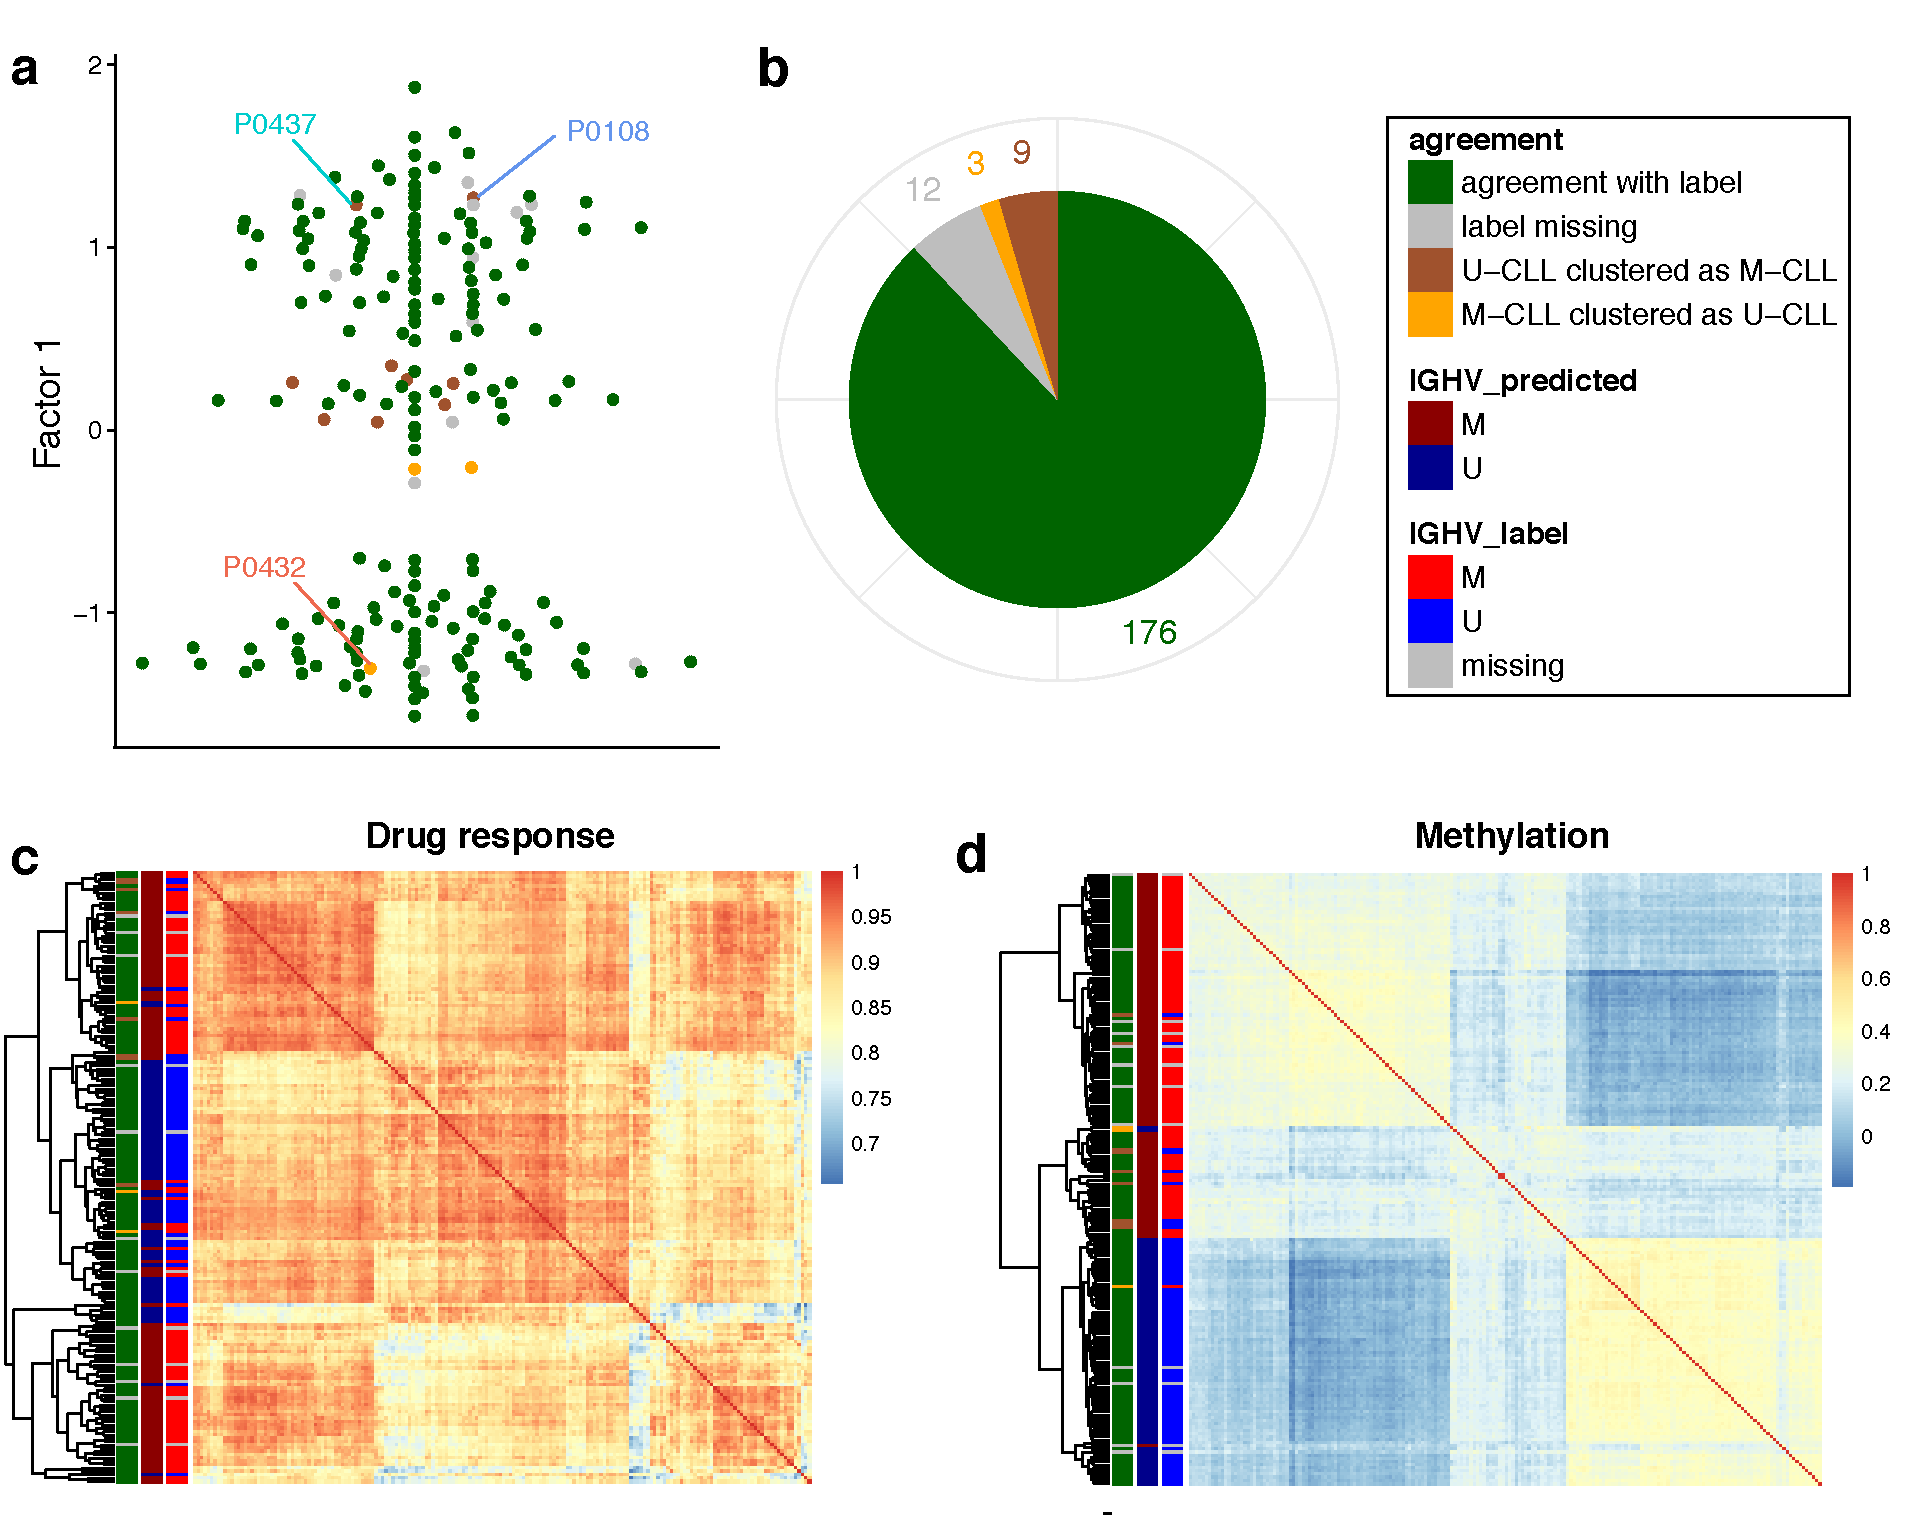
\includegraphics[width=1.0\textwidth]{MOFA_IGHV_outlier}
% 	\caption{XX}
% 	\label{fig:MOFA_IGHV_outlier}
% \end{figure}

\subsubsection{Molecular characterisation of Factor 1}
% \tabularnewline

An important step in the MOFA pipeline is the characterisation of the molecular signatures underlying each Factor. I will demonstrate this for Factor 1, although a similar strategy can be applied to Factor 2.

On the RNA expression, inspection of the top weights pinpoint genes that have been previously associated to IGHV status, some of which have been proposed as clinical markers\cite{Vasconcelos2005,Morabito2015}. Heatmaps of the RNA expression levels for these genes reveals clear differences between samples when ordinated according to the Factor 1 values.

On the drug response data the weights highlight kinase inhibitors targeting the B-cell receptor pathway. Splitting the patients into three groups based on k-means clustering shows clear separation in the drug response curves.

% Copied
\begin{figure}[H]
	\centering 	
	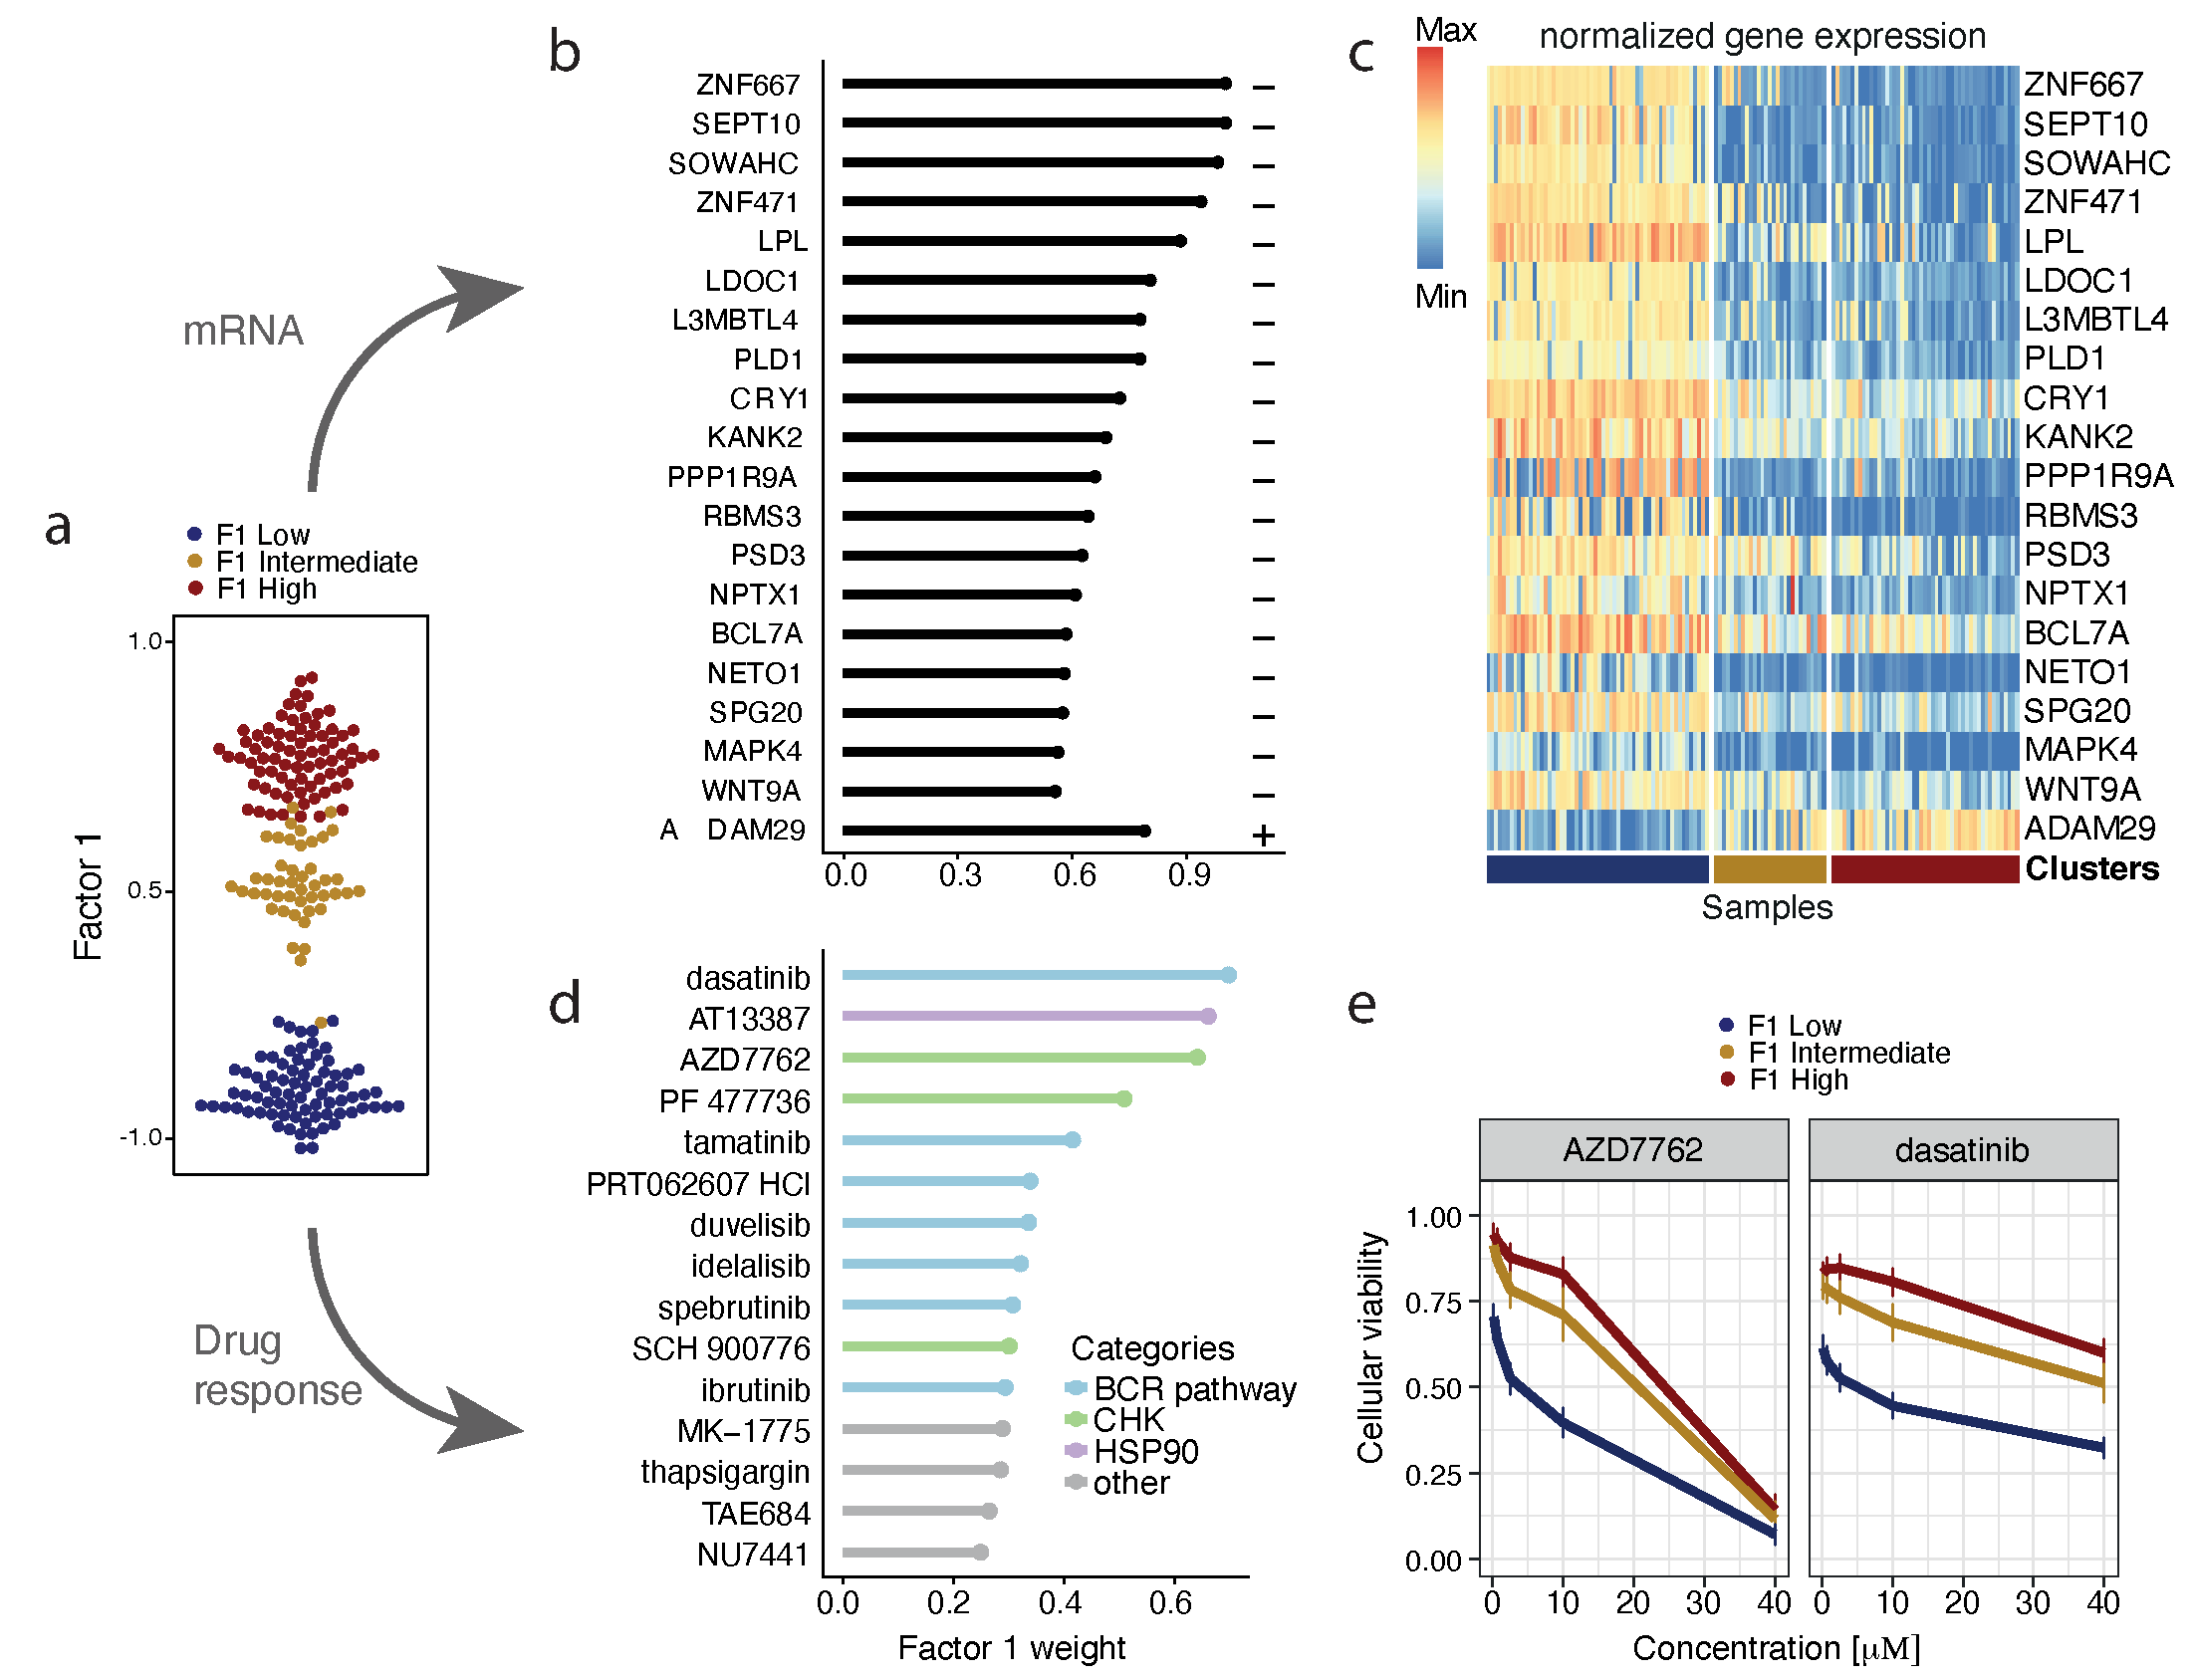
\includegraphics[width=0.90\textwidth]{MOFA_CLL_Factor1}
	\caption{
	\textbf{Characterization of MOFA Factor 1 as IGHV status.}\\
	(a) Beeswarm plot with Factor 1 values for each sample with colours corresponding to three groups found by 3-means clustering with low factor values (LZ), intermediate factor values (IZ) and high factor values (HZ).\\
	(b) Absolute weights for the genes with the largest absolute weights in the mRNA data. Plus or minus symbols on the right indicate the sign of the loading. Genes highlighted in orange were previously described as prognostic markers in CLL and associated with IGHV status (Vasconcelos et al, 2005; Maloum et al, 2009; Trojani et al, 2012; Morabito et al, 2015; Plesingerova et al, 2017).\\
	(c) Heatmap of gene expression values for genes with the largest weights as in (b).\\
	(d) Absolute weights of the drugs with the largest weights, annotated by target category.\\
	(e) Drug response curves for two of the drugs with top weights, stratified by the clusters as in (a).
	}
	\label{fig:MOFA_CLL_Factor1}
\end{figure}

\subsubsection{Characterisation of other Factors}

Despite their clinical importance, Factor 1 (IGHV status) and Factor 2 (chr12 trisomy) they explain less than 20\% variability in each data modality, suggesting the existence of more subtle sources of variation. As an example, we will also characterise Factor 5, which explains 2\% of the variance in the mRNA and 6\% of variance in the drug response.\\
As mentioned in \Cref{mofa:downstream}, instead of exploring the feature weights individually, factors can be annotated using gene set annotations. This procedure is particularly appealing for RNA expression data, as a rich amount of resources exist that have categorised genes into ontologies in terms of biological pathways, molecular function and cellular components  \cite{Fabregat2015,Ashburner2000}.\\
Briefly, the idea is to aggregate the weights using prior information to obtain a single statistic for each gene set, which can be tested against a competitive null hypothesis. Inspired from \cite{Frost2015}, in MOFA we implemented several scoring schemes and a variety of parametric and unparametric statistical tests. We refer the reader to \cite{Frost2015} for details.

Appling Gene Set Enrichment Analysis on the RNA weights using the Reactome annotations \cite{Fabregat2015} reveals that Factor 2 is strongly enriched for oxidative stress and senescence pathways. Inspection of the top features highlights the importance of heat shock proteins (HSPs), a group of proteins that are essential for protein stability which are up-regulated upon stress conditions like high temperatures, pH shift or oxidative stress. Importantly, HSPs can be elevated in tumour cells and potentially contribute to prolonged tumour cell survival\cite{Dempsey2010}.\\
In agreement with the findings from the mRNA view, the drugs with largest weights on Factor 5 belong to clinical categories associated with stress response, such as target reactive oxygen species (SD07, MIS-43, SD51) and DNA damage response (fludarabine, nutlin-3, doxorubicine) (Figure S12c-d).

% All together, our results indicate that blood cells from patients with high expression of HSPs display higher viability to the aforementioned drugs.

% Copied
\begin{figure}[H]
	\centering 	
	\includegraphics[width=0.95\textwidth]{MOFA_CLL_Factor5}
	\caption{
	\textbf{Characterization of Factor 5 in the CLL data as oxidative stress response.}\\
	(a) Beeswarm plot of Factor 5. Colours denote the expression of TNF, an inflammatory stress marker that is present among the top RNA weights.\\
	(b) Gene set enrichment analysis for the top Reactome pathways. Displayed are the top pathways with the strongest enrichment in the RNA weights. P-values were adjusted for multiple testing using the Benjamini-Hochberg procedure.\\
	(c) Heatmap of mRNA expression values for representative genes with the largest weights. Samples are ordered by their factor values.\\
	(d) Scaled weights for the top drugs with the largest loading, annotated by target category.\\
	(e) Heatmap of drug response values for the top three drugs with largest weight.
	}
	\label{fig:MOFA_CLL_Factor5}
\end{figure}


\subsubsection{Prediction of clinical outcomes}

We conjectured that the integration of multiple molecular layers could allow an improved prediction of the patients' clinical outcome.\\
To evaluate the utility of the MOFA factors as predictors of clinical outcomes we fit Cox regression models \cite{Cox1972} using the patients' time to next treatment (TTT) as a response variable. Two types of analysis were performed: a univariate analysis where each Factor was independently associated with TTT, and a multivariate analysis where the combination of all Factors were used to predict TTT (\Cref{fig:MOFA_CLL_Cox}).\\
In the univariate Cox models, we observe  that Factor 1 (IGHV status), Factor 7 (associated with chemo-immunotherapy treatment prior to sample collection) and Factor 8 (enriched for Wnt signalling) were significant predictors of TTT. Accordingly, when splitting patients into binary groups based on the corresponding Factor values, we observe clear differences in the survival curves.\\
In the multivariate Cox model, MOFA (Harrell's C-Index C=0.78) outperformed all other input settings, including PCA on single-omic data (C=0.68-0.72), individual genetic markers (C=0.66) as well PCA applied to the concatenated data matrix (C=0.74).

%As predictors, we included the top 10 principal components calculated on the data for each single view, a concatenated data set ('all') as well as the 10 MOFA factors. Missing values in a view were set to the feature-wise mean. 

% Caption copied
\begin{figure}[H]
	\centering 	
	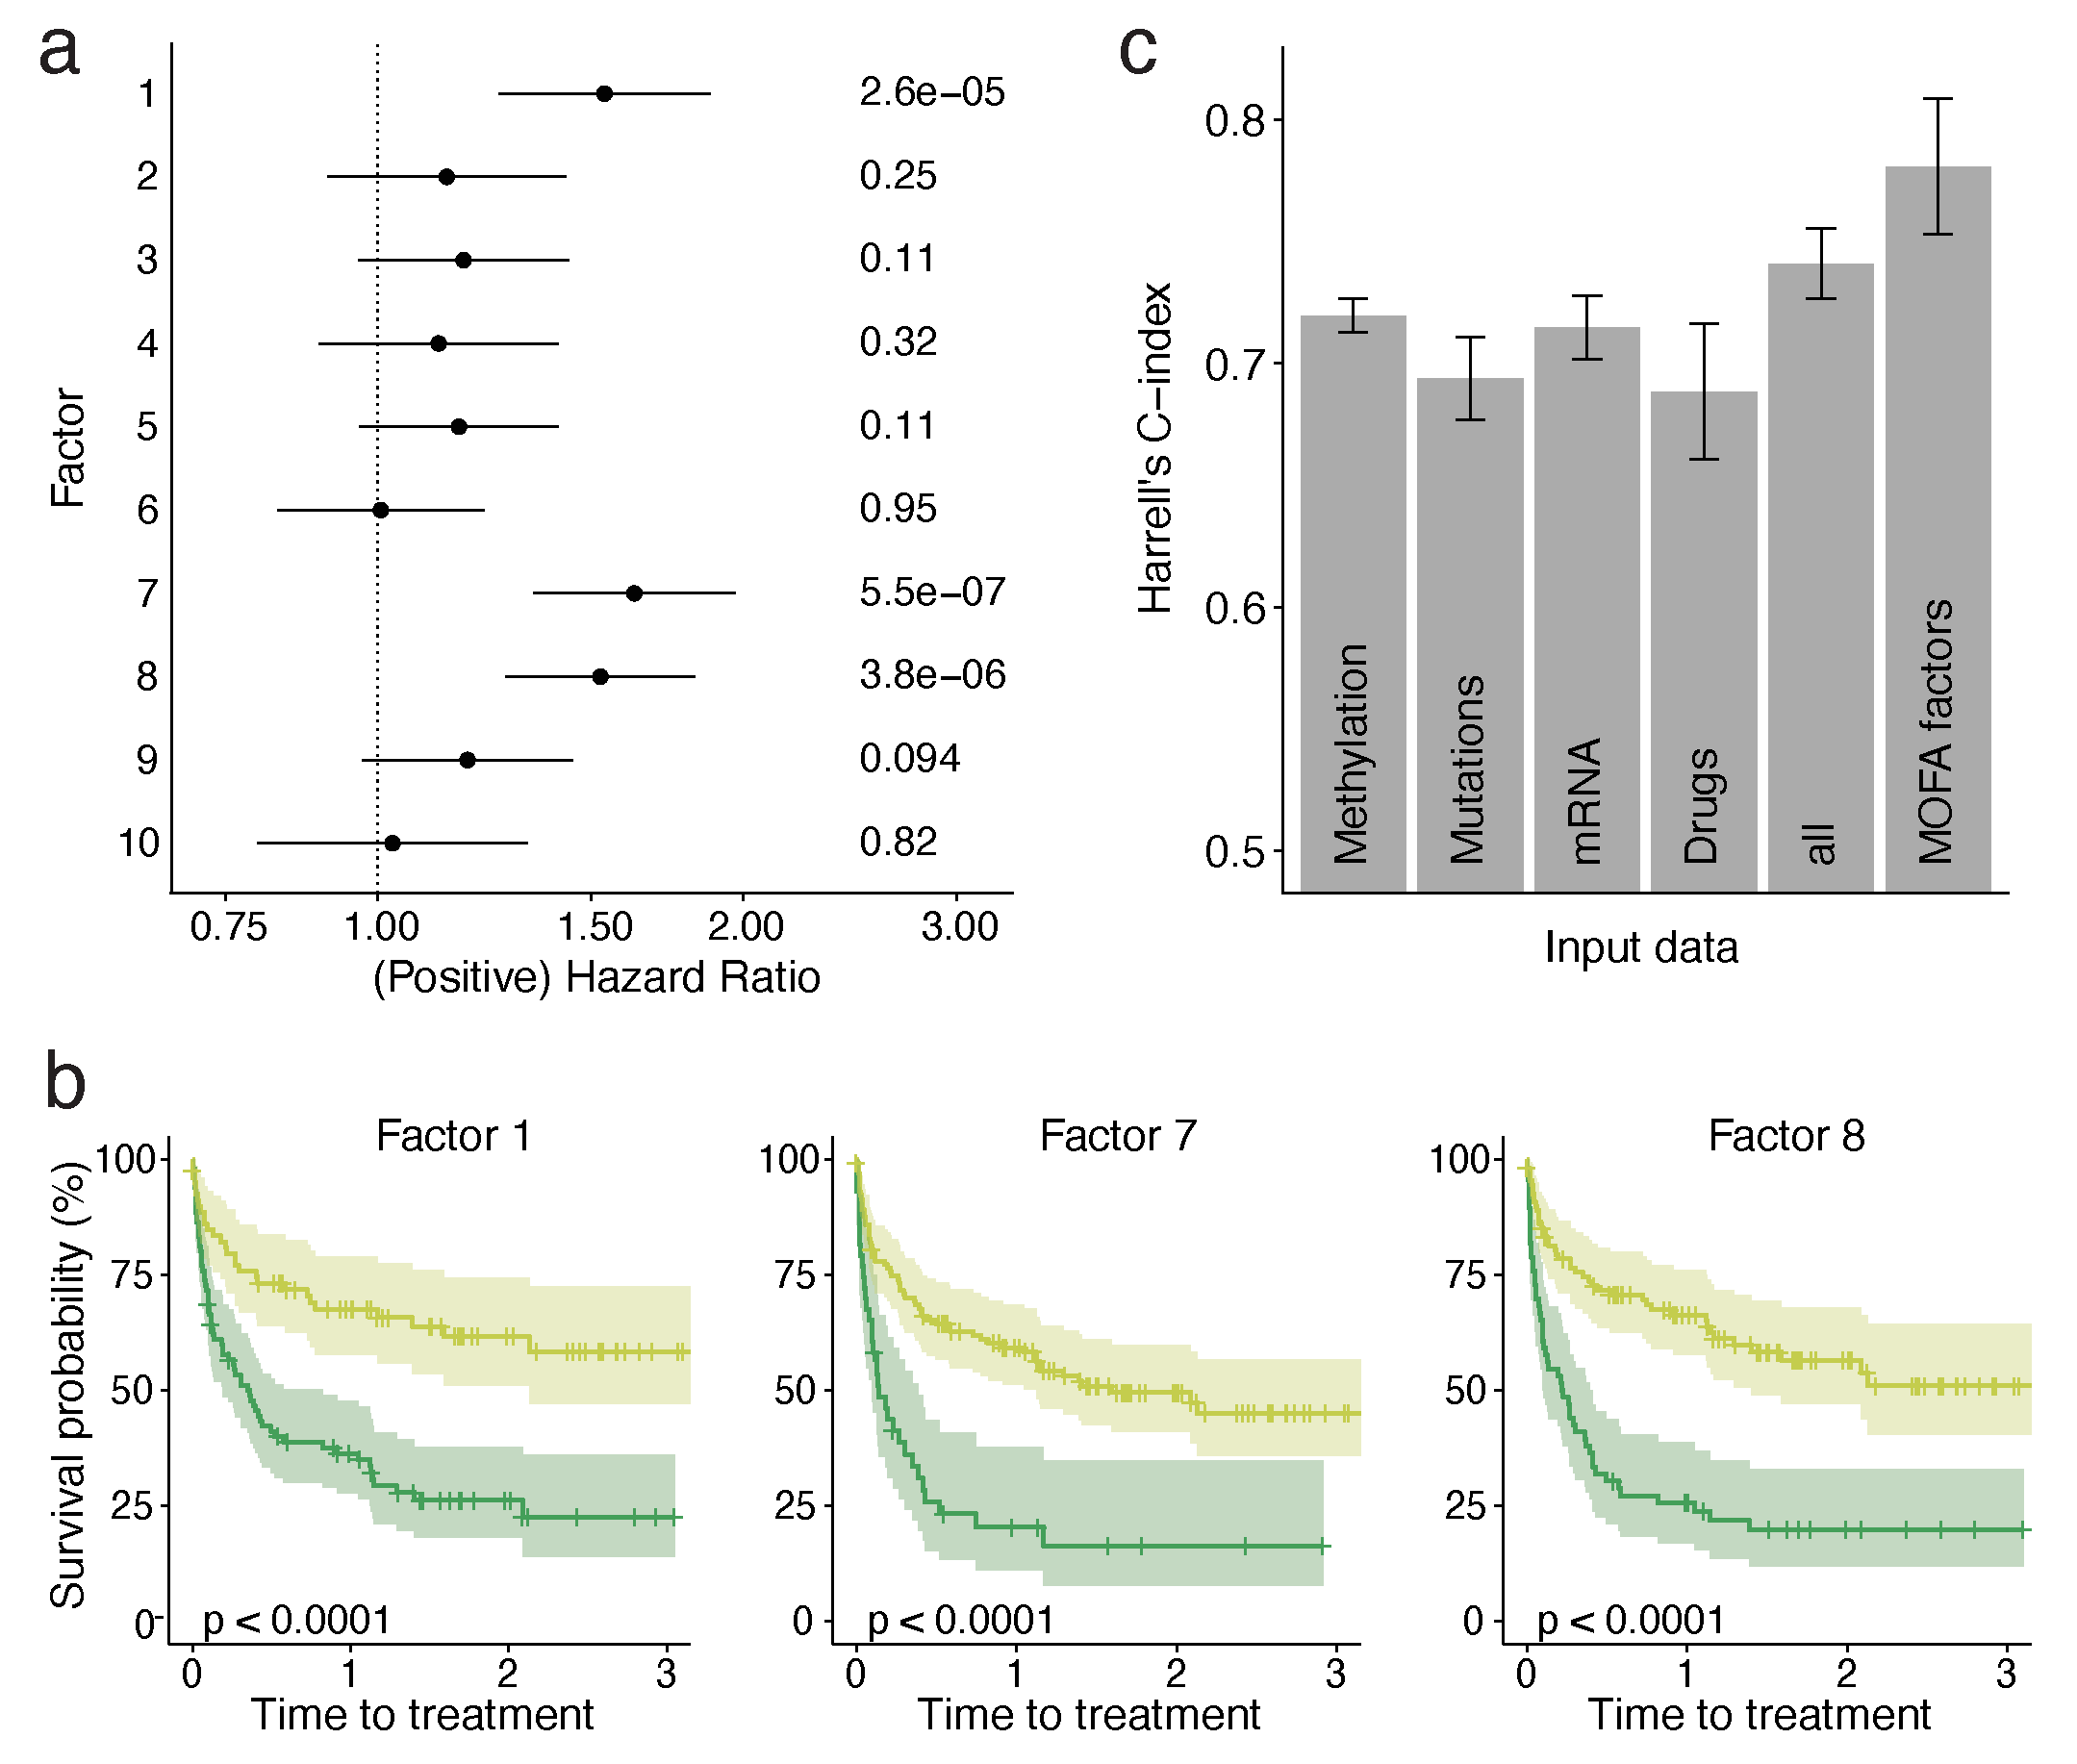
\includegraphics[width=0.9\textwidth]{MOFA_CLL_Cox}
	\caption{
	\textbf{Association analysis between MOFA Factors and clinical putcome.}\\
	(a) Association of MOFA factors to time to next treatment using a univariate Cox regression with N = 174 samples (96 of which are uncensored cases) and p-values based on the Wald statistic. Error bars denote 95\% confidence intervals. Numbers on the right denote p-values for each predictor.\\
	(b) Kaplan-Meier plots measuring time to next treatment for the individual MOFA factors. The cut-points on each factor were chosen using maximally selected rank statistics, and p-values were calculated using a log-rank test on the resulting groups.\\
	(c) Prediction accuracy of time to treatment for N = 174 patients using multivariate Cox regression trained with the 10 MOFA factors, as well using the first 10 principal components applied to single data modalities and the full data set. Shown are average values of Harrell's C-index from fivefold cross-validation. Error bars denote standard error of the mean.
	}
	\label{fig:MOFA_CLL_Cox}
\end{figure}


\subsubsection{Imputation of missing values}

A promising application of MOFA is the imputation of missing values, including the potential to impute of entire assays.\\
The principle of imputation in MOFA follows the same logic as simulating from the generative model: if the factors and weights are known, the input data can be reconstructed by a simple matrix multiplication:
\[
	\hat{\bfY} = \E[\bfZ] \E[\bfW]^T
\]
where $\E[\bfZ]$ and $\E[\bfW]$ denote the expected values of the variational distributions for the factors and the weights, respectively. Notice that, when using the expectations of the posterior distributions, the noise $\epsilon$ (\Cref{mofa_master_equation}) has a mean of zero and does not contribute to the predictions.\\
The equation above computes a point estimate for every sample $n$ and feature $d$, but it ignores the uncertainity on $\bfZ$ and $\bfW$. Instead of relying in point estimates, one could adopt a more Bayesian approach and calculate the posterior predictive distribution by propagating the uncertainity \cite{Gelman2013}. Nonetheless, due to the nature of the optimisation problem in variational inference, the variance of the posterior distributions can be underestimated (see \Cref{section:expectation_propagation}). In addition, this would more complex to implement and would result in a significant increase in computational complexity. 
Hence, and also because of the additional computational complexity, we did not attempt this approach.

To assess the imputation performance, we trained MOFA models using a data set of complete measurements (a total of N=121 samples) after masking parts of the drug response measurements. In a first experiment, we masked values at random, and in a second experiment we masked the entire drug response measurements. We compared the imputation accuracy of MOFA to some established imputation strategies, including imputation by feature-wise mean, SoftImpute \cite{Mazumder2010}, a k-nearest neighbour method \cite{Troyanskaya2001}.\\
For both imputation tasks, MOFA consistently yielded more accurate predictions, albeit the differences are less pronounced in the imputation of full assays, a significantly more challenging task.

\begin{figure}[H]
	\centering 	
	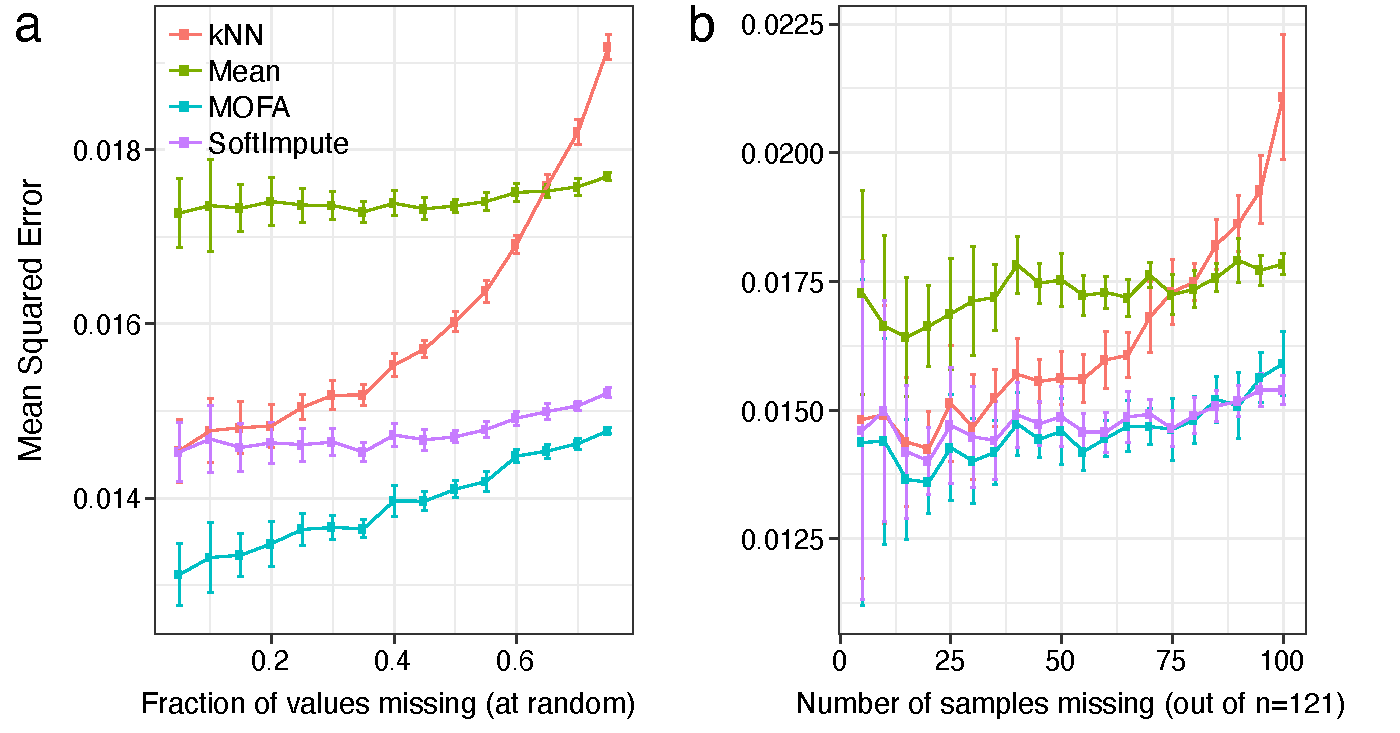
\includegraphics[width=1.0\textwidth]{MOFA_imputation}
	\caption{\textbf{Evaluation of imputation performance in the drug response assay.}\\
	The y-axis shows the mean-squared error (MSE) across 15 trials for increasing fractions of missing data (x-axis). Two experiments were considered: (a) values missing at random and (b) entire assays missing at random. Each point displays the mean across all trials and the error bars depict the corresponding standard deviations.}
	\label{fig:MOFA_imputation}
\end{figure}

\newpage

\subsection{Application to single-cell multi-omics} \label{section:mofa_scmt}

The emergence of single-cell multi-modal techniques has created open opportunities for the development of novel computational strategies \cite{Stuart2019,Colome-Tatche2018,Chappell2018}.\\
To show case how MOFA can be used to integrate single-cell multi-omics data, we considered a simple data set that consists on 87 ESCs where RNA expression and DNA methylation were simultaneously measured using single-cell Methylation and Transcriptome sequencing (scM\&T-seq)\cite{Angermueller2016}. Two populations of ESCs were profiled: the first one contains 16 cells grown in 2i media, which is known to induce a native pluripotency state associated with genome-wide DNA hypomethylation \cite{Ficz2013}. The second population contains 71 cells grown in serum media, which contain stimuli that trigger a primed pluripotency state poised for differentiation \cite{Tosolini2016}.

\subsection{Data processing}

The RNA expression data was processed using \textit{scran}\cite{Lun2016b} to obtain log normalised counts adjusted by library size. Feature selection was performed by selecting the top 5,000 most overdispersed genes\cite{Lun2016a}. A Gaussian likelihod was used for this data modality. \\
The DNA methylation data was processed as described in Chapter 1. Briefly, for each CpG site, we calculated a binary methylation rate from the ratio of methylated read counts to total read counts. Next, CpG sites were classified by overlapping with genomic contexts, namely promoters, CpG islands and enhancers (distal H3K27ac peaks). Finally, for each annotation we selected the top 5,000 most variable CpG sites with a minimum coverage of 10\% across cells. Each of the resulting matrices was defined as a separate view for MOFA. A Bernoulli likelihod was used for this data modality.


\subsubsection{Model overview}

In this data set, MOFA inferred 3 factors with a minimum explained variance of 1\% (\Cref{fig:mofa_scMT}). Factor 1 captured the transition from naive to primed pluripotent states, which MOFA links to widespread coordinated changes between DNA methylation and RNA expression. Inspection of the gene weights for Factor 1 pinpoints important pluripotency markers including  \textit{Rex1/Zpf42} or \textit{Essrb} \cite{Mohammed2017}. As previously described both \textit{in vitro} \cite{Angermueller2016} and \textit{in vivo} \cite{Auclair2014}, the transition from naive to primed pluripotency state is concomitant with a genome-wide increase in DNA methylation levels. Factor 2 captured a second dimension of heterogeneity driven by the transition from a primed pluripotency state to a differentiated state, with RNA weights enriched with canonical differentiation markers including keratins and annexins \cite{Fuchs1988}.\\
Jointly, the combination of Factors 1 and 2 reconstruct the coordinated changes between the transcriptome and the epigenome along the differentiation trajectory from naive pluripotent cells to differentiated cells.

\begin{figure}[H]
	\centering 	
	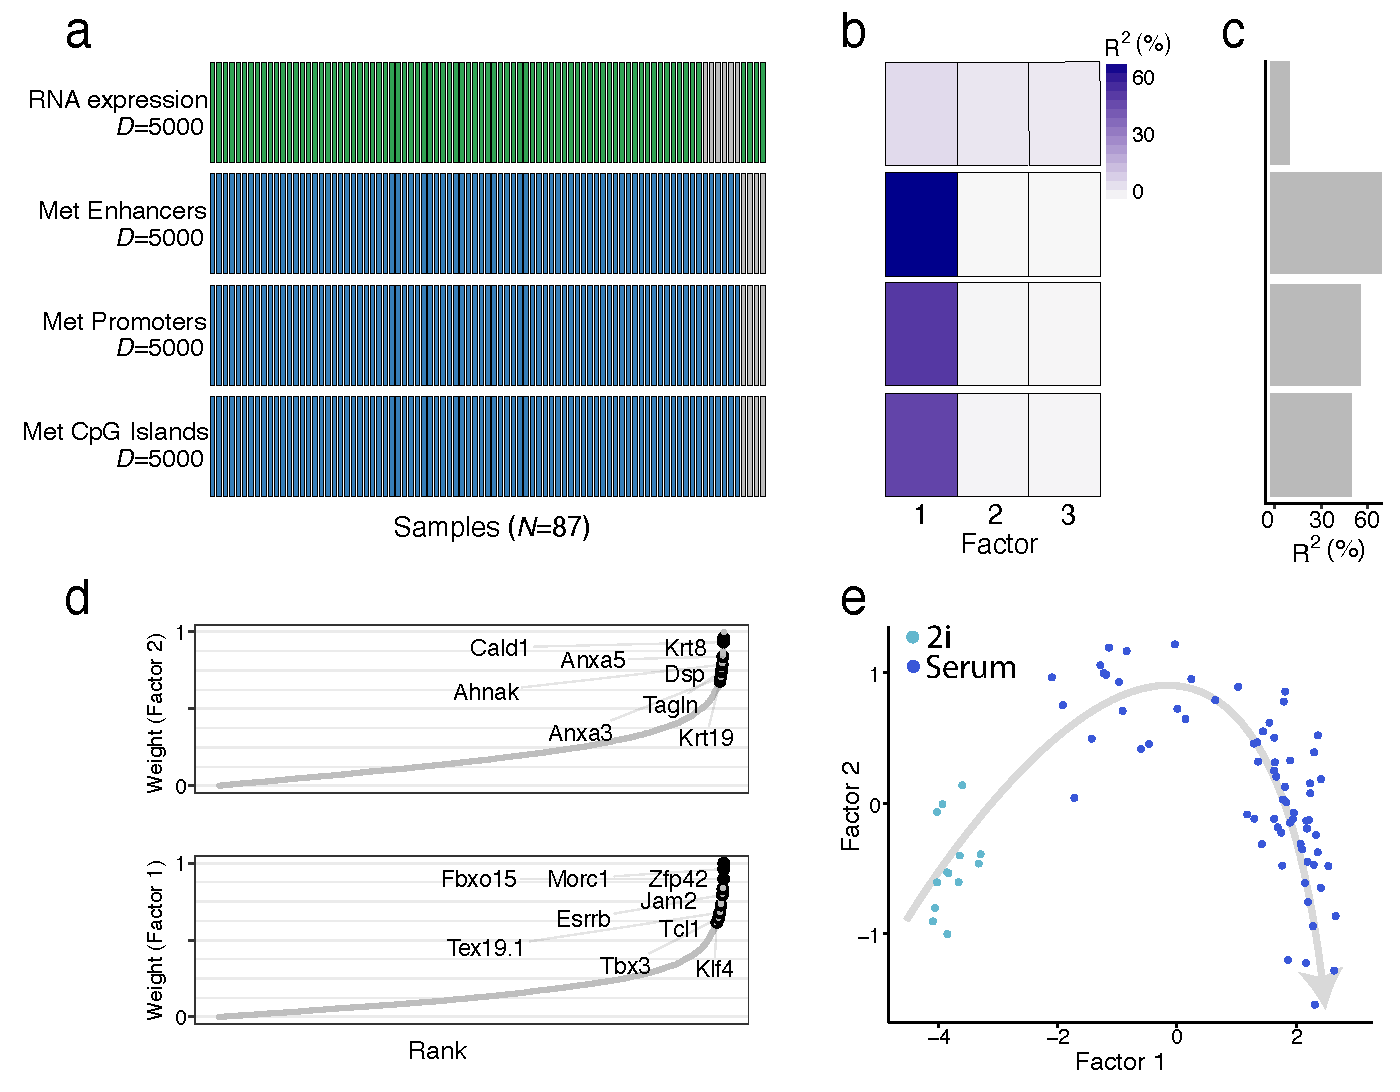
\includegraphics[width=0.9\textwidth]{MOFA_scMT}
	\caption{\textbf{MOFA recovers a differentiation process from a single-cell multi-omics data set.} \\
	(a) Overview of the data modalities. Rows indicate number of features ($D$) and columns indicate number of samples ($N$). Grey bars denote missing samples.\\
	(b) Fraction of variance explained per factor (column) and view (row).\\
	(c) Cumulative fraction of variance explained per view (across all factors).\\
	(d) mRNA weights of Factor 1 (bottom) and Factor 2 (top). The genes that are labelled are known markers of pluripotency (for Factor 1) or differentiation (for Factor 2). \\
	(e) Scatter plot of Factor 1 (x-axis) against Factor 2 (y-axis). Cells are colored based on the culture condition. Grey arrow illustrates the differentiation trajectory from a naive pluripotency state to a differentiated state. 
	}
	\label{fig:mofa_scMT}
\end{figure}

% \begin{figure}[H]
% 	\centering 	
% 	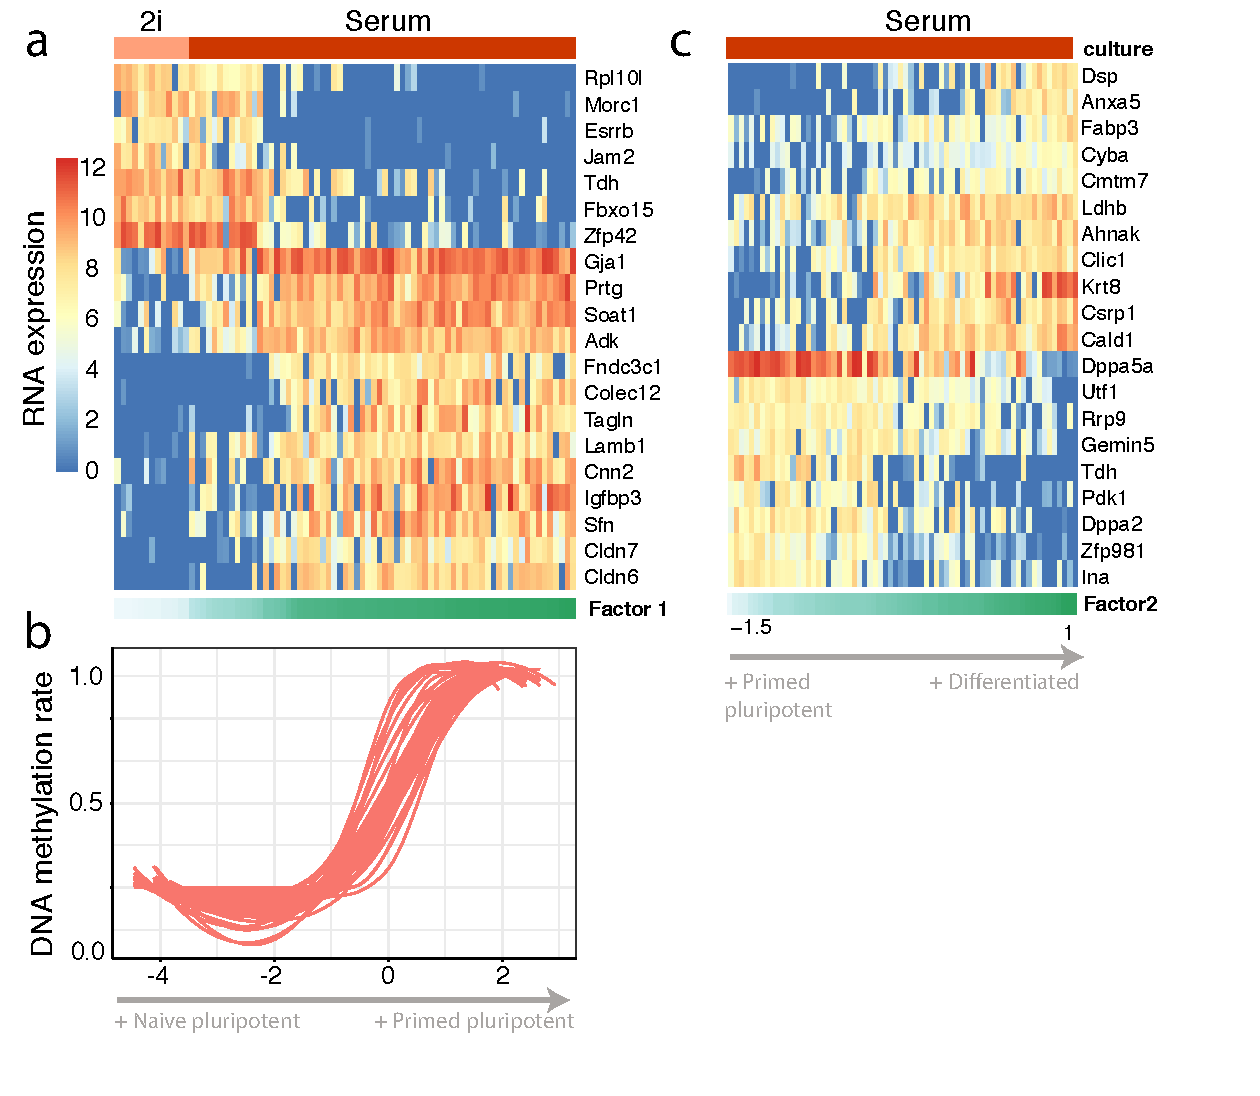
\includegraphics[width=0.8\textwidth]{MOFA_scMT2}
% 	\caption{XX}
% 	\label{fig:MOFA_scMT2}
% \end{figure}

% \subsubsection{Comparison with clustering strategies}

% To illustrate the importance of learning continuous latent spaces before clustering samples, we applied popular integrative clustering algorithms \cite{Wang2014,Shen2009,Mo2013} to the data set. As expected, two clusters can be recovered that broadly match the culture conditions. However, no trajectory is recovered, illustrating the importance of 

% \begin{figure}[H]
% 	\centering 	
% 	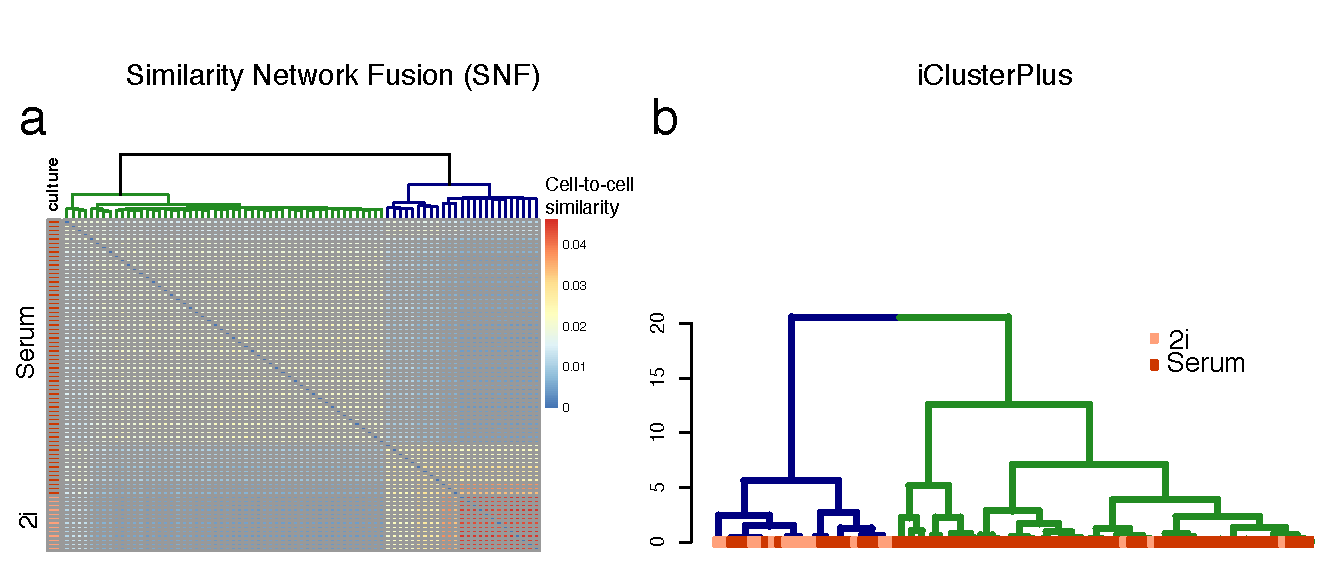
\includegraphics[width=1.0\textwidth]{MOFA_scMT_clustering}
% 	\caption{\textbf{Multi-omics clustering applied to scMT data set.}\\
% 	(a) Similarity matrix and dendogram obtained using Similarity Network Fusion\cite{Wang2014}\\
% 	(b) Dendrogram obtained using iClusterPlus\cite{Mo2013} with two clusters.
% 	}
% 	\label{fig:MOFA_scMT_clustering}
% \end{figure}


\newpage

\subsection{Limitations and open perspectives}

MOFA solves important challenges for the integrative analysis of (single-cell) multi-omics data sets. Yet, the model is not free of limitations and there are open possibilities for future research:

\begin{itemize}

	\item \textbf{Linearity}: this is an assumption that is critical for obtaining interpretable feature weights. Nonetheless, there is a trade-off between explanatory power and interpretability\cite{Kuhn}. Non-linear approaches, including deep neural networks or variational autoencoders have shown promising results when it comes to dimensionality reduction \cite{Lin2017,Ding2018,Lopez2018}, batch correction\cite{Lopez2018}, denoising \cite{Eraslan2019} or imputation \cite{Lin2016}. Interestngly, very few multi-view factor analysis models exist that incorporate flexible non-linear assumptions, making it an interesting line of research to explore.

	\item \textbf{Scalability}: the size of biological datasets is rapidly increasing, particularly in the field of single cell sequencing \cite{Svensson2018,Cao2019}. \\
	When comparing the inference framework to previous methods that make use of sampling-based MCMC approaches, the variatonal framework implemented in MOFA yields a vast improvement in scalability. Yet, in its vanilla form, variational inference also becomes prohibitively slow with very large datasets \cite{Hoffman2013,Blei2016,Hoffman2014}. This has been recently addressed by a reformulation of the variational inference problem in terms of a gradient descent optimisation problem, which enables the full machinery of stochastic inference to be applied in the context of Bayesian inference.
	%hence motivating the development of even more efficient inference schemes that potentially scale to milions of samples. 
	%This line of research is followed in Chapter 4, with the development of a stochastic version of the variational inference algorithm.

	\item \textbf{Generalisations to multi-group structures}: the sparsity assumptions in MOFA are based on the principle that features are structured into non-overlapping views. As such, the activity of the latent factors is also expected to be structured, so that different factors explain variability in different subsets of views (\Cref{fig:MOFA}). Following the same logic, many studies contain structured samples, as either multiple experiments or conditions. A simple generalisation of MOFA would be to intuitively break the assumption of independent samples and introduce an additional prior that captures the group structure at the sample level.

	\item \textbf{Tailored likelihoods for single-cell analysis}: MOFA enables the modular extension to arbitrary non-gaussian likelihoods, provided that they can be locally bounded and integrated into the variational framework (see \Cref{section:mofa_ngaussian}). New likelihood models such as zero-inflated negative binomial distributions \cite{Risso2018} could make MOFA more suited to the analysis of single-cell data.

	\item \textbf{Bayesian treatment of predictions}: in the current implementation of MOFA, only the point estimates for the posterior distributions are used in the downstream analysis. While convienient for most operations, this ignores the uncertainity associated with the point estimates, which is a major strength of Bayesian modelling. Future extensions could attempt a more comprehensive Bayesian treatment that propagates uncertainity in the downstream analyses, mainly when it comes to making predictions and imputation \cite{Gelman2013}.

	\item \textbf{Incorporation of prior information}: an unsupevised approach is appealing for discovering the principal axes of variation, but sometimes this can yield challenges in the interpretation of factors. Future extensions could exploit the rich information encoded in gene set ontologies, similar to the methodology proposed in \cite{Buettner2017}.

\end{itemize}


